\documentclass[12pt, a4]{scrartcl}

\usepackage[utf8]{inputenc}
\usepackage[T1]{fontenc}    % use 8-bit T1 fonts
\usepackage{url}            % simple URL typesetting
\usepackage{booktabs}       % professional-quality tables
\usepackage{amsfonts}       % blackboard math symbols
\usepackage{nicefrac}       % compact symbols for 1/2, etc.
\usepackage{microtype}      % microtypography
\usepackage{lipsum}
\usepackage[svgnames]{xcolor}
\usepackage[linewidth=1pt]{mdframed}
\usepackage{graphicx}
\usepackage{array}
\usepackage{imakeidx}

\nonstopmode

\deffootnote[1em]{1em}{1em}{\textsuperscript{\thefootnotemark}}

\graphicspath{ {images/} }

\title{Severe Influenza Pandemic in the Macaronesian Islands:}
\subtitle{Preparedness and Response}


\author{Lucas González Santa Cruz} \\

\date {December 15, 2011}
\makeindex

\begin{document}
\maketitle

\footnotesize { \centering
Creative Commons License “Attribution-Noncommercial-Share Alike”
\\
\\

\includegraphics[height=2em,width=2em]{license/cc.eps} 
\includegraphics[height=2em,width=2em]{license/by.eps} 
\includegraphics[height=2em,width=2em]{license/nc.eps} 
\includegraphics[height=2em,width=2em]{license/sa.eps}

} \\   % Creative Commons license

\newpage
\\
\\
\textbf{Author:} Lucas González Santa Cruz
\\
\\
\textbf{Version:} December 15, 2011 \\
\textbf{Translation and updates:} March 17, 2013\\
\textbf{LaTeX Conversion:} March 13, 2020\\
\\
\\
\textbf{License:} This work, including the attachments, is licensed under Creative Commons “Attribution Noncommercial: Share Alike” 2.0 England and Wales. 
\\
\\
\textbf{Financing:} Gestión de Servicios para la Salud y Seguridad de Canarias (Management of Services for Health and Safety in the Canaries, GSC, a public company of the Canary Islands, attached to the Canary Islands Ministry of Presidency, Justice and Security, and to the Ministry of Health), under the PLESCAMAC2 project (Health Emergency Plan in case of Disaster in the Macaronesia 2, Activity 6, specific objective 2), within the Transnational Cooperation Programme Madeira-Azores-Canaries (MAC) 2007-2013.
\\
\\
\textbf{Acknowledgments:} This work is based in part on Dealing in Security (understanding vital services and how they keep you safe), Vinay Gupta, published under Creative Commons “Attribution-Noncommercial-Share Alike” license 2.0 England \& Wales. It is also based in part on the OODA loop by Colonel John Boyd (USAF). The author would like to thank Elizabeth Sweet for her invaluable assistance as copy editor for the English translation.
\\
\\
\textbf{Abbreviations:}
\begin{itemize}
	\item WHO: World Health Organization http://www.who.int
	\item ECDC: European Center for Disease Control http://www.ecdc.eu
	\item CDC: Centers for Disease Control and Prevention of the United States http://www.cdc.gov
	\item SCIM: Simple Critical Infrastructure Maps http://ResilienceMaps.org
	\item OODA: Observation, Orientation, Decision and Action loop
\end{itemize}
\newpage

\printindex

\newpage
\section{Introduction}
History shows that, over the last few centuries, at irregular intervals of one to several decades, there have been a dozen influenza pandemics, some of which have caused an elevated number of influenzarelated deaths and resulted in socio-economic disruption as they swept through populations. The most catastrophic pandemic within this period has been that of 1918-19, which killed tens of millions of people globally, many of them young and previously healthy.

In recent years, various viruses among the many that cause influenza in animals have occasionally produced disease in humans, but only in the case of 2009 H1N1 has the sustained interhuman transmission that would lead to a new pandemic been observed. Other strains have sometimes infected humans, but have yet to be transmitted easily from one person to another. Among these, the H5N1 virus has caused illness in more than 600 people, of whom nearly 60\% have died. The presence of these viruses in wild ecosystems makes it unlikely that they will disappear, and our current knowledge of the mechanisms of pandemic emergence does not enable us to predict when the next influenza pandemic will emerge or what virus will cause it. Therefore the possibility of a highly lethal pandemic cannot be ruled out.

For the development of pandemic scenarios, a pandemic in which 1\% of patients die is considered to be severe. A 1\% fatality rate would mean that, if 30\% of the population were to fall ill, as has happened historically during influenza pandemics, then 300,000 people per million inhabitants would fall ill and, of these, 3,000 would die from complications of influenza. (History shows worse possibilities.) But a severe and disruptive influenza pandemic may well also claim the lives of people who never catch the virus. When pandemic influenza infection rates soar, many among the workforce may be sidelined by illness or caretaking responsibilities. The systemic disruptions that may result, cascading through supply chains and services, are discussed in detail in section II.4 on “Impact of a severe pandemic”. Thus, to deaths from pandemic influenza we would have to add deaths incurred as a result of the disruption of vital services and supplies (including medical ones).

Faced with the threat of a deadly and disruptive pandemic, global preparations intensified after 2005. There were improvements in coordination between countries and regions as well as in epidemiological and virological surveillance, and the production of vaccines was streamlined. The evidence about the benefits of the tools available to reduce infections was reviewed, and health-care contingency plans and recommendations to essential businesses were drawn.

These activities have lost a measure of momentum after the 2009-10 pandemic, partly due to the worsening global economic situation. On the other hand, virological research and slow technological progress in vaccines persist, and international organizations continue to explore the involvement of sectors beyond those specifically dealing with health care.

This document summarizes the knowledge and strategies already in place, and proposes a framework for agile and flexible response by civil protection and essential services facing a severe pandemic — a framework that could be useful in other crises, from non-pandemic origins but equally broad in terms of geography and systemic impact. It is accompanied by spreadsheets to facilitate the development of scenarios and plans, and by a presentation for the training of at least an initial number of civil protection and essential services staff.

The material is published under an open license, to allow and encourage its distribution, use, and improvement. 

\textbf{Note: }This LaTeX document was created by Jason Brink (http://www.rubricpartners.io) for the purpose of making this document easier to translate and disseminate in a time when this sort of thinking may be important. No attempt to assert ownership or authorship is being made. Please forgive any errors in transcription as this was done in something of a hurry. If you see any errors, please feel free to make a pull request with corrections. I have updated a number of the source links as many of them linked to dead pages. Efforts have been made to make sure that the exact document had been duplicated elsewhere, but I really have no way of knowing. Also, please forgive the formatting. I am far from an expert in LaTeX, but I wanted to do what I could to help. Stay healthy!
\newpage
\section{Pandemic Challenge}
\begin{mdframed}[leftmargin=10pt,rightmargin=10pt]
\begin{itemize}
	\item Influenza pandemics have historically emerged at intervals of one to several decades.
	\item We know many details regarding influenza viruses and the mechanisms by which human pandemics emerge from viruses adapted to animals, but we are unable to predict which virus will cause the next pandemic, or when.
	\item Some pandemics have produced high mortality rates, particularly the pandemic of 1918-19, which caused a high number of deaths among previously healthy young adults.
	\item That is why we keep monitoring influenza viruses (such as the H5N1 strain) which, while well-adapted to animals, have also occasionally caused disease in people.
\end{itemize}
\end{mdframed}

\subsection{The biology of influenza}
To understand the pandemic potential of influenza and the apparent inevitability of pandemics, we must first look at key features of the influenza virus, the animal species in which the different strains of the virus are found, the mechanisms by which new varieties appear, and how influenza spreads.

\subsubsection{Influenza Viruses}
Flu viruses are unable to replicate autonomously. Their surface contains molecules of hemagglutinin (H) which enable them to adhere to the surface of the cell, which they are then able to penetrate. Once the virus invades, the cell replication system creates new copies of the virus, which leave the cell using other surface molecules (neuraminidase, N).

There are three types of influenza viruses (A, B and C). Type B has no subtypes. Winter influenza is presently caused by three variants: A(H1N1), A(H3N2) and B. Only type A has proved capable of causing pandemics, which is why the rest of this document refers only to type A.

The type A virus is categorised into subtypes, named according to their hemagglutinin and neuraminidase variants: H1N1, H3N2, H5N1, and many others.

\begin{figure}[h]
\centering
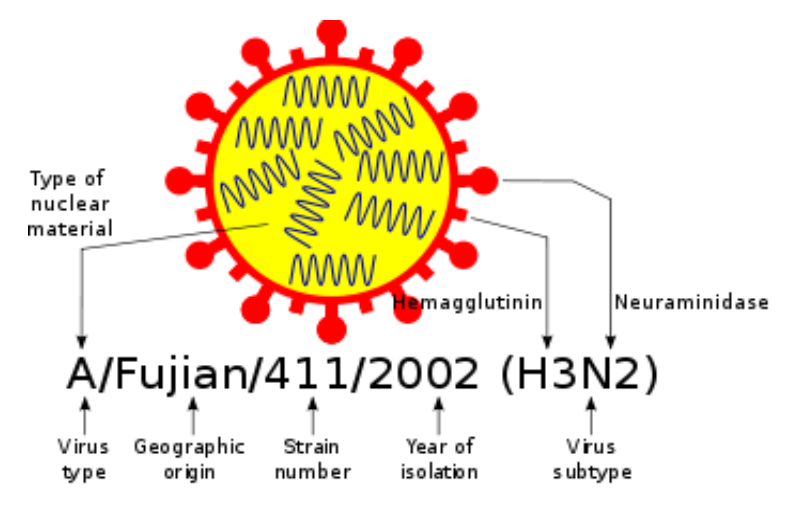
\includegraphics[width=8cm]{/figs/fig1.png}
\caption{Naming of influenza viruses. Source: Wikipedia.}
\end{figure}

\subsubsection{Mutation and hybridization}
Viral replication within a cell has no effective mechanism of “quality control”, so it is relatively frequent that some copies are different from the original. Many of those imperfect copies are not viable. Most of the viable ones result in viruses functionally identical to their parent. 

In some cases, however, mutations involve the acquisition of new capabilities of some importance, such as being resistant to the previous year's vaccination or to antiviral treatment. 

In rare but important cases, the mutation generates a virus substantially different from their parents, maybe able to invade a species different from that to which it was originally adapted. Thus, it was an avian virus that led to the pandemic of 1918-19, which resulted in the order of 50 million deaths within a world population of 1,800 million people.

The second known mechanism by which new influenza viruses have emerged is hybridization, which occurs when an animal – a pig, for instance – has a dual infection (e.g., by one virus adapted to humans and by another virus adapted to birds). In this case, the genetic material of both viruses may be present in the same cell at the time of replication, allowing the emergence of a genetically mixed virus.

The pandemics of 1957-58, 1968-69 and 2009-10 – each of which caused a much lower mortality than that of 1918-19, and more similar to seasonal flu – were caused by hybrid viruses. A case in point, the H1N1 virus that resulted in the 2009-10 pandemic contained genetic material from influenza viruses adapted to humans, pigs and poultry.

\begin{figure}[h]
\centering
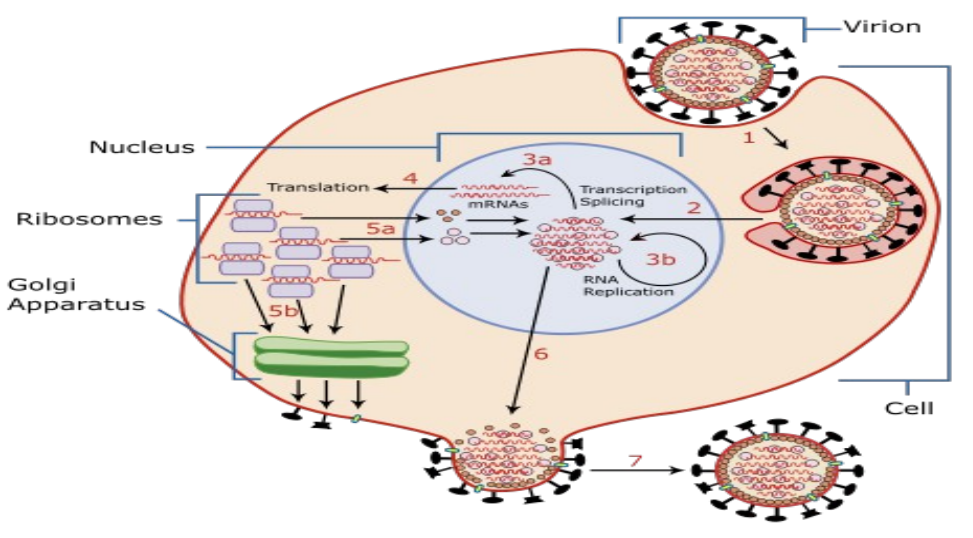
\includegraphics[width=12cm]{/figs/fig2.png}
\caption{Reproductive cycle of influenza viruses. Source: Wikipedia.}
\end{figure}

\subsubsection{Animal species}
The two mechanisms mentioned (mutation and hybridization) explain the large variability of influenza viruses, of which only a small number of known subtypes are capable of infecting mammals, such as pigs, cats, horses, dogs and even bats.

Most subtypes are found in birds (especially waterfowl, in which the flu spreads through the digestive tract and produces mild or asymptomatic infections). In poultry there are viruses characterized by low pathogenicity (which cause mild infections) and highly pathogenic viruses (which kill a high percentage of the infected birds, up to 80\% or higher). It has been observed that viruses of low pathogenicity can mutate, acquiring high pathogenicity. Among avian viruses, H5N1 – as we will see in more detail later –is a highly pathogenic virus in poultry that continues to produce large losses in affected countries, where it has killed or forced the culling of more than 500 million birds in the last decade.

\subsubsection{Transmissibility}
Although influenza in waterfowl is transmitted through the digestive tract, in poultry it is transmitted by inhalation or by direct contact. 

Human seasonal and pandemic influenzas are likewise transmitted by inhalation and through contact with contaminated surfaces. Transmission is more common during the early stages of infection, even before symptoms first appear (incubation period), and to a lesser extent from people who have asymptomatic infections.

Regarding animal-to-human influenza (such as H5N1), until now primary transmission (from bird to human) has occurred in situations of direct intense exposure.

Secondary transmission (from one infected person to another) has been very limited. Apparently, one reason might be that, when inhaled, the viruses which are adapted to birds attach themselves to cell membrane receptors abundant only in the deeper portions of the human respiratory system. Since a person must inhale the virus deeply in order for it to reach those receptors, person-to-person transmission of avian viruses is difficult. Human winter influenza viruses, however, are adapted to attach to receptors abundant in the upper, more accessible, portions of the respiratory system, facilitating more effective person-to-person transmission. It is speculated that, in order for a new influenza virus to cause a pandemic, it must first acquire the ability to bind to respiratory cells in the upper portions of the human respiratory tract.

\subsection{History of pandemics}
To understand the history of influenza pandemics, we will first review how they emerge and unfold. Then we will examine pandemics of recent centuries, concluding with special attention to the 1918-19 pandemic.

\subsubsection {Development of a pandemic}
A subtype of an influenza virus, one that’s new to humans, emerges as a result of mutation or hybridisation. Given the appropriate attributes and conditions, that virus can start spreading from person to person in a more or less explosive way, causing epidemic waves worldwide.

These waves repeat themselves for one or two years until finally most of the human population has been exposed to the virus, which then can no longer qualify as “new”. Unlike winter influenza, which generates a single annual wave at some point in the “flu season” \footnote{In the northern hemisphere, influenza season goes from week 40 (first week of October) until week 20 next year (mid-May).}, pandemic influenza may cause more than one wave per year, at any time of the year, with waves one to several months apart from each other.

In each wave, the majority of cases would occur in the weeks of the epidemic peak \footnote{In the Annexes (see section VII.2), a spreadsheet is provided in which initial parameters can be typed (population, proportion of the population that would fall ill, proportion of those ill who would die) in order to compute the likely number of ill and the likely number of deaths, and their distribution along weeks for a given scenario.} proposed by the experts from the UK suggest that, out of every million people, 40,000 to 80,000 may fall ill each week during the peak of a pandemic wave \footnote{https://www.wp.dh.gov.uk/publications/files/2012/11/SPI-M-Modelling-Summary-15_06_12.pdf}.

The number of cases to be expected during a pandemic wave may be much higher than would be caused by seasonal influenza; thus case volume would affect primary care services. If, in addition, a significant proportion of the cases proved to be severe, hospital services would be affected, and all this at a time when a percentage of health care workers (or their families) would also be affected by illness. 

It should be noted that – for both seasonal and pandemic influenza – each general wave (in a country, for example) is actually the sum of local waves (regions, for example), which are not synchronous but rather begin and end at different times. So every local wave is shorter and more intense than the general one, which is, in actuality, a “summary” wave.

\subsubsection {Attack rate, lethality, mortality and hospitalization rates}

In a pandemic, the attack rate, or the proportion of the population that has symptomatic influenza, can be several times higher than is the case with seasonal influenza. But, as with seasonal influenza, the attack rate for pandemic influenza is generally higher among people less than 20 years of age and lower among those who are over 65.

In “mild” pandemics (similar in severity to winter influenza), lethality, or the proportion of patients who die, has been greater in those over 65, in people with chronic diseases, and in pregnant women. (Age, chronic disease, and pregnancy are all “risk factors”.) Notably, compared with seasonal flu, the 2009-10 pandemic caused more severe disease in young people, in those with known risk factors, and in those with marked obesity (with a body mass index greater than 40). Mortality is the result of multiplying attack rate and lethality. So if 30\% of the population falls ill and 1\% of patients die, mortality would be 3,000 per million.

For the hospital system the proportion of patients who become candidates for admission would be very important. We would generally expect numbers of hospital admissions to be several times higher than numbers of deaths.

\subsubsection {Pandemics in past centuries}
Historians \footnote{Potter, CW (October 2006). “A History of Influenza”. J Appl Microbiol. 91 (4): 572–579. doi:10.1046/j.1365-2672.2001.01492.x. PMID 11576290.} have agreed to classify as pandemics worldwide epidemics that unfolded as successive waves with symptoms compatible with influenza. History indicates that pandemics swept across the globe in 1580, 1694, 1729, 1781, 1830 and 1898. Twentieth century pandemics occurred in 1918-19, 1957-58 and 1968-69, and the first pandemic of the twenty-first century unfolded in 2009-10.

Thus, we can say pandemics have occurred at a rate of at least one to three per century (two to three in recent centuries), at intervals of one or more decades. Pandemics have been very different from each other. Recent history shows that the pandemics of 1957-58, 1968-69 and 2009-10 could be classified as “mild”, while those of 1918-19 and 1830 were far
more severe.

\subsubsection {The 1918-19 pandemic}
Of all the pandemics known to history, the 1918-19 pandemic resulted in the highest mortality\footnote{1918 Influenza: the Mother of All Pandemics. Jeffery Taubenberger, David Morens.
http://wwwnc.cdc.gov/eid/article/12/1/05-0979_article.htm}. In a time when the world population numbered about 1,800 million people, an estimated 50 million lives were lost to pandemic influenza. (Given the current world population of more than 7,000 million people, a similar level of mortality today would translate to 195 million deaths.)

The lethality of the 1918-19 pandemic is often estimated to be 2\%. However, if the attack rate, more difficult to estimate than the mortality, was around 30\% as in more recent pandemics, then the actual lethality would have been just over 9 deaths per 100 patients, or >9\%. In any case, both figures are higher than 1\%, the lower limit that would define a severe pandemic. Mortality caused by the 1918-19 pandemic showed some other special features. First, the number of deaths was much higher in the second wave than in the first. This has made experts think that the virus might have mutated after the first wave to become more deadly and/or more contagious. 

Second, the lethality rate was disproportionately high in previously healthy 20-40 year-old adults. In some very isolated places such as Alaska, mortality was very high in almost all ages except in children. Because of these two facts, three hypotheses have been suggested: that a pandemic some 50 years earlier had been caused by a similar virus which protected the elderly in 1918-19, that children were protected by a distinct immunological reactivity, and/or that young adults exhibited an extreme immune response that was harmful in itself (a “cytokine storm”)\footnote{Protective immunity and susceptibility to infectious diseases: lessons from the 1918 influenza pandemia. Rafi Ahmed, Michael BA Oldstone, Peter Palese. http://www.nature.com/ni/journal/v8/n11/pdf/ni1530.pdf and http://www.nature.com/ni/journal/v8/n11/fig_tab/ni1530_F3.html}.

\begin{figure}[h]
\centering
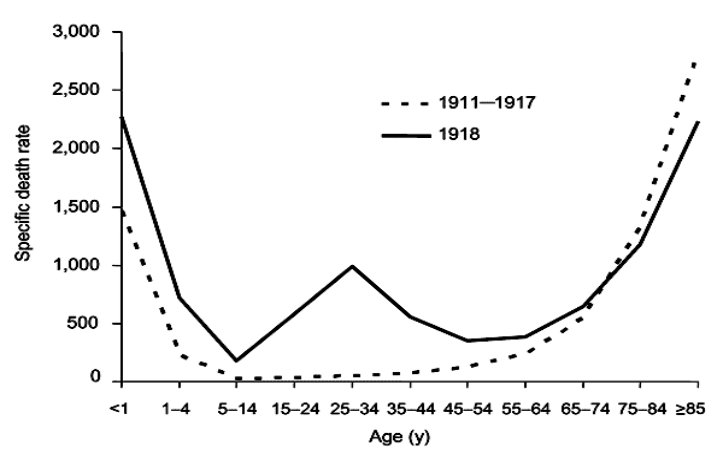
\includegraphics[width=12cm]{/figs/fig3.png}
\caption{Age-specific lethality in the 1918-19 pandemic. Source: Taubenberger, J; Morens D (2006). “1918
Influenza: the mother of all pandemics”. Emerg Infect Dis 12 (1): 15-22}
\end{figure}

\subsection {Animal-human influenza – H5N1}
\subsubsection{Pandemic candidates}
Viruses with the greatest potential to cause pandemics are believed to be those which infect domesticated animals, such as pigs and poultry, that are frequently in close contact with humans. Of these, of particular concern are those viruses that have produced disease in people, especially when it seems likely that a virus has been transmitted from one person to another.

Several influenza viruses meet these criteria to a greater or lesser extent: H9N2, some variants of H7 (N2, N3 and N7), H10N7 and H5N1\footnote{Avian influenza (Bird Flu): implications for human disease. CIDRAP. http://www.cidrap.umn.edu/cidrap/content/influenza/avianflu/biofacts/avflu_human.html}. For example, a H7N7 outbreak occurred in 2003 in the Netherlands, with 89 human cases, one death, and a number of asymptomatic infections.

In 1997 in Hong Kong, an H5N1 epidemic in poultry resulted in 18 human cases of the disease, including 6 deaths. Between 1997 and 2003, no human cases of H5N1 were detected. But in late 2003, the virus returned to produce epidemics in poultry\footnote{H5N1 epidemics in birds have happened in several continents. We would not term these widespread avian epidemics a “pandemic” (as we would with humans) but rather a “panzootic”} associated with occasional human cases, and since then it has become a persistent problem.

\subsubsection {H5N1’s lethality}
H5N1 has so far caused at least 603 human cases with at least 356 deaths\footnote{ http://www.who.int/influenza/human_animal_interface/H5N1_cumulative_table_archives/en/index.html May, 2 2012}, many of them in children and young people, previously healthy\footnote{Avian Influenza A (H5N1) Age Distribution in Humans. Emerg Infect Dis. 2007 March; 13(3): 510–512.}.

Cases have been detected in a dozen countries, with significant differences in mortality. In Indonesia, for example, 80\% of cases have died, whereas in Egypt 40\% have died. These differences may be due to different detection systems, or to characteristics of the virus itself, which has mutated in the last decade to give rise to more than 20 “clades” (virologically distinct variants). 

Beyond the number of confirmed cases, the possible existence of cases with mild or no symptoms has been explored. It is difficult to interpret the results of these studies for methodological reasons, but the current consensus among scientists is that H5N1 produces few mild cases\footnote{http://www.cidrap.umn.edu/cidrap/content/influenza/avianflu/news/mar1312seroprev.html}, although there are scientists who think otherwise\footnote{Seroevidence for H5N1 Influenza Infections in Humans: Meta-analysis. Taia T Wang, Michael K Parides, Peter Palese. http://www.sciencemag.org/content/early/2012/02/22/science.1218888.abstract}. Again, the genetic variability of the virus is invoked to explain why different studies – considered poor by all authors – see different frequencies for markers of previous infection.

\subsubsection {Secondary Cases}
H5N1 has caused a number of cases where person-to-person transmission is considered very likely. In some situations it is difficult to distinguish between parallel transmission (from one bird to two humans) and a true secondary transmission (from bird to a person and then from that person to another). The longest chain of transmission documented to date took place in Peshawar (Pakistan) in December 2007: a first human case – infected from sick birds – infected another person, the second infected a third, and the third infected a fourth\footnote{http://www.who.int/csr/don/2008_04_03/fr/} (see also III.2.a, “detecting the start of a pandemic”).

\begin{figure}[h]
\centering
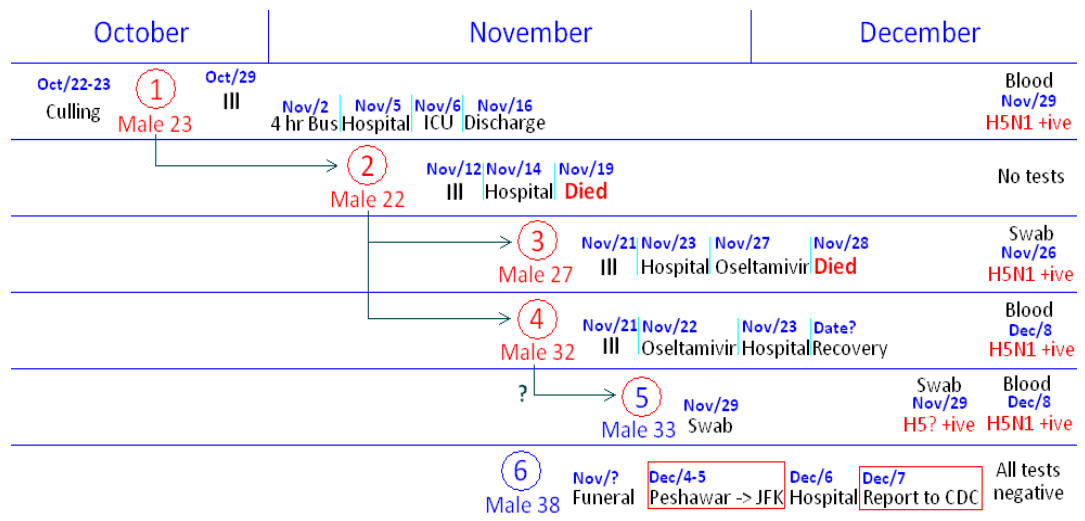
\includegraphics[width=15cm]{/figs/fig4.png}
\caption{Human transmission of H5N1 in Peshawar (Pakistan), December 2007}
\end{figure}

\subsubsection{Possible futures}
We cannot know what the next influenza pandemic will be like in terms of contagiousness and severity, or when it will start. It may happen 30 years from now, or later or sooner than that; and it may be comparable in its lethality to the relatively mild pandemics of 1957-58, 1968-69 and 2009-10 – or to the deadly pandemic of 1918-19, or even worse.

Depending on how long we have before the next pandemic emerges and on how fast scientific and technological advances can be made in the interim, it is possible that vaccines or treatments may have improved to the point where they can be produced abundantly and quickly, substantially reducing the disruption a pandemic would otherwise cause in a complex world of more than 7,000 million people.

Based on what we know of animal-human influenza and the history of pandemics, and based on the fact that we currently lack adequate means to blunt the impact of spreading infection, experts and health authorities insist that it is not reasonable to drop our guard. Among the avian influenza viruses that may pose a pandemic threat is the highly lethal H5N1 virus.

An overview of what we know about it follows:

\begin{itemize}
\item The persistence of H5N1 in wild birds (some of them migratory) makes the disappearance of the virus unlikely. This fact, the appearance of genetically distinct variants of the virus, and documented existence of limited inter-human transmission all mean that we cannot rule out H5N1 as “pandemic candidate”.
\item Recent research with ferrets\footnote{The publication of those papers was delayed in January 2012 while experts debated the risks posed by “double use technology,” which might serve not only to advance scientific knowledge but also to enable the development of a biological weapon. The danger of an accidental escape from the laboratories constituted another security concern. The first study was finally published in May 2nd, 2012 http://www.nature.com/nature/journal/vaop/ncurrent/full/nature10831.html, and the second one in June 22nd, 2012 http://www.sciencemag.org/content/336/6088/1534.full.} animals considered a good model for human transmissibility, suggests that, with several transmissions from one animal to another, the virus may acquire the ability to spread through the respiratory route with the same ease as seasonal influenza. In the natural environment, H5N1 has reached, as far as we know, a maximum of 4 instances of humanto-human transmission (the situation already mentioned in Peshawar, 2007).
\end{itemize}

It remains to be seen whether the virus, should it acquire the ability to spread easily, would retain its current lethality. If, for example, lethality were to be reduced to a tenth of that observed to date, mortality would still be potentially very high.

Finally, as we assess the potential impacts of an influenza pandemic, we must keep in mind that a pandemic need not be highly lethal in order to result in disproportionately intense social disruption. This would probably be the case if the mortality were “intermediate” (between 1/10³ and 1/10²) in ages for which deaths rarely occur. For example, if 30\% of the 5 to 20 year olds become ill, and 0.5\% of those who fall ill die, then the mortality in this age group would be 150 per 100,000 children and adolescents, a figure that, in developed countries where child mortality is low, would be several times higher than the annual death rate in this age range, but concentrated in a small number of weeks\footnote{Given the population of the Canary Islands in 2006, as an example, 106,081 of the 353,603 5 to 20 year olds would get sick, and 530 would die – 6.5 times the number (81) who died in that age group in 2006.}.

\subsection {Impact of a severe pandemic}

\begin{mdframed}[leftmargin=10pt,rightmargin=10pt]
\begin{itemize}
	\item A severe pandemic would cause illness, death, and disruption.
	\item In a severe influenza pandemic, deaths would be caused not only by the disease itself, but also by the disruption of essential services and supplies.
	\item The interaction between different factors – deaths, infection avoidance measures, and socio-economic and health-care disruption – would make a severe pandemic qualify as
a complex process.
\end{itemize}
\end{mdframed}

\subsubsection {Severity factors}
A pandemic can be severe for two reasons.

First, by the ability of the virus itself to produce, in a substantial proportion of individuals, more or less severe disease. This ability depends on several factors, not all well known:

\begin{itemize}
	\item It's likely that there are features of the virus that enable it multiply faster within cells.
	\item Features of the immune system, which in part of the population would behave in a poorly regulated way (sometimes called “cytokine storm”), have also been invoked.
	\item As discussed in Section 2, on the history of pandemics, mortality tends to occur more frequently in certain groups (the elderly, those with certain chronic diseases, and pregnant women). But in 1918-19 there was a disproportionate mortality among previously healthy young adults (20-40 years of age).
\end{itemize}

In addition to what happens at the individual level, a pandemic’s severity as an epidemiological, health-care, and social phenomenon will depend on other factors\footnote{http://www.who.int/csr/disease/swineflu/assess/disease_swineflu_assess_20090511/en/index.html Assessing the severity of an influenza pandemic. May 11 2009.}:

\begin{itemize}
	\item The characteristics of the epidemic as such (not only its lethality but also the proportion of the population that falls ill, the rate at which cases appear, the lethality by age group, and so on), and 
	\item The response capacity both in the health-care system (such as organization of health services and effectiveness and availability of medications) and in the whole of society (such as organization of prevention and vulnerability to disruption).
\end{itemize}

\subsubsection {An illustrative scenario}
In 2007, the CDC published its Pandemic Severity Index\footnote{http://www.pandemicflu.gov/planning-preparedness/community/commitigation.html}, suggesting that a pandemic would be categorised as “mild” if the fatality rate (proportion of deaths among patients) were similar to that observed for seasonal influenza, and therefore less than one death per thousand ill (<1/10³ or <0.1\%). It would be categorised as “severe” (levels 4-5 out of 5) if lethality were to exceed one percent (>1/10² or >1\%), and “intermediate” (levels 2-3 out of 5) if it were to fall between those two values.

The ECDC, based on data from the twentieth century pandemics, suggested a pandemic scenario with an attack rate of 30\%. The number of severe cases (those who would be candidates for hospitalization) would be many times the number of deaths, exceeding the usual hospital resources.

\begin{figure}[h]
\centering
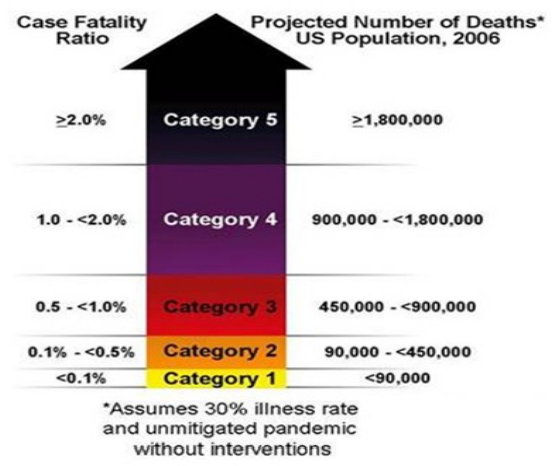
\includegraphics[width=12cm]{/figs/fig5.png}
\caption{Pandemic Severity Index suggested by the Center for Disease Control in the United States in 2007. Source:
http://www.flu.gov/planning-preparedness/community/mitigation.html.}
\end{figure}

To illustrate the possible impact of a severe pandemic, a scenario could be constructed with an attack rate of 30\%, a lethality rate of 1\% – at the lower end of the “severe” range as assessed by CDC’s Severity Index – and, for each fatality, four cases serious enough to be candidates for hospitalization. In that situation, among 100 people, 25 would have relatively mild disease, 4 serious illness, and 1 fatal disease – in other words, per million people, 40,000 would need hospitalisation and 10,000 might die.

The proportion of the population that would be affected, even if 30\% on average, would probably differ by age group. For the purposes of planning, figures of 40\% for those under 20 years, and 20\% for those over 65 have been suggested.

We can use different attack rates and fatality rates to explore alternative scenarios, using the spreadsheet attached as an annex. The CDC has publicly used a lethality of 10\%, consistent with estimates of how the 1918-19 pandemic behaved globally, with a lethality that might have been greater than 9\%\footnote{World population in 1918 was 1,800 million people. Estimates suggest that the 1918 pandemic caused a grand total of 50 million deaths. With an attack rate 30\%, lethality would have been greater than 9\%}.

\subsubsection{Direct and indirect effects in a severe pandemic}
Direct effects from pandemic influenza are the disease itself (mild or severe), and deaths. The remaining effects are indirect, and may be directly proportional to the direct ones, or they may feed on themselves and have a disproportionate impact.

In a severe pandemic (with a lethality of at least 1\%, historically possible with influenza), it is reasonable to assume that a high proportion of the population would be \emph{interested in avoiding infection}, partly for themselves and partly so that they wouldn't infect those around them (family, friends, neighbors, co-workers, and others), some of whom might be especially vulnerable because of known risk factors.

Workplace \emph{absenteeism} during a pandemic will derive from workers being ill or needing to care for sick family members, from deaths, and from attempting to protect their households and themselves from infection by staying home from work, keeping children home from school and otherwise minimizing contacts outside the home. Absenteeism can be expected among all occupational groups, and rates of absenteeism may soar or attenuate depending on the moment within the pandemic wave. Absenteeism among health-care workers (highest at times of greatest need because health-care workers and their families would be affected along with everyone else), civil protection workers, and supply transport workers would have the greatest impact on the welfare of society as a whole. In general, absenteeism would be disproportionately harmful in skilled jobs, so that, for example, surgery would be difficult if the entire team is present except for the anesthetist.

In a severe pandemic, disease, death and interest in avoiding infection would also cause “\emph{customer absenteeism}”: consumers in general and especially travelers (tourists and professionals) can be expected to reduce consumption of non-vital goods and services to gain in security. The result would be a significant economic contraction. Econometric modeling has shown that the economic impact would derive mostly from avoidance behaviours rather than from the direct effects of influenza (including deaths). It has been estimated that the economic impact could be pronounced, with a reduction of 0.7\% of GDP for a pandemic causing 2.5 million deaths, and up to 5\% of GDP (or more) for a pandemic causing 70 million deaths\footnote{http://web.worldbank.org/WBSITE/EXTERNAL/NEWS/0,,contentMDK:20979352~pagePK:64257043~piPK:437376~th eSitePK:4607,00.html “Avian flu: the economic costs.” Milan Brahmbhatt, World Bank, June 2006, Paris}.

Absenteeism among transport workers might cause, to a greater or lesser degree, \emph{supply failures}. Compounding any supply problem is the fact that shortages (or even the mere perception of possible shortages) tend to alarm consumers, particularly in just-in-time delivery systems. Those who are able to stock up would do so more or less simultaneously, leaving less for others and thereby further compounding supply problems. Fuel shortages, in particular, would impact transportation systems themselves and, in turn, the timely distribution of everything else. Shortages of specialized material resources, such as spare parts for repairs, or certain raw materials, would affect the entire production chain. Finally, supply issues with key medical supplies might arise, as the demand for antivirals, antibiotics, masks, respirators and similar resources would be simultaneously intense in many countries.

Absenteeism among health workers and among those who transport medical equipment and supplies could cause “\emph{health-care system insufficiency}” to the extent that the health-care system might not able to meet all the needs of the population. Of particular concern would be adequate care of diseases and conditions with potential for serious complications (births, heart attacks, serious injuries and so on), and chronic diseases requiring a steady supply of vital medications (such as insulin-dependent diabetes, cancer and others). Mortality from such conditions, usually “contained” by the health-care system, would become partially “uncontained” in a severe pandemic, and this indirect effect of a pandemic would increase the total number of deaths. The potential number of deaths secondary to disruption of medical services and supplies would be different in each place. For example, there are populations in which 3,000 out of every million people are insulin-dependent diabetics.

Absenteeism among those who produce and transport other types of vital supplies, and economic contraction, could cause shortages of food, water or products needed to treat water and make it drinkable. Such shortages may in turn result in localized resource conflicts. All of this may ultimately increase mortality figures in percentages that would be variable and difficult to predict.

A severe pandemic, by definition, would incur one or more of the consequences mentioned, although each of them might occur in varying degrees in each place and in each moment.

\subsubsection{Complex global crises}

In summary, illnesses and deaths from influenza would cause health-care and socio-economic disruption, possibly in a non-linear fashion with respect to mortality, and this disruption would in turn have the potential to produce even more deaths.

Behaviors that \emph{amplify} disruption would certainly be offset by behaviors that have the potential to contain it, to the extent that people – perhaps in an organized and facilitated way – resolve to “go to work anyway”, and find that they must “buy essentials anyway”. This compensatory tendency would be partial and dynamic, varying with perceived risk, such that levels of disruption will likewise vary according to time and place.

Moreover, all this disruption may be mitigated by coordinated action. The effectiveness of coordinated action, however, will be compromised to some degree by actions taken by “not well-coordinated agents” (other countries, people within the same country). Such uncoordinated actions would cause a detrimental effect on even the most farsighted and effectively orchestrated mitigation measures.

These systemic failure loops are what turn a severe pandemic into a crisis not only global in scope, but also complex in its development.

Since this would be a global crisis, it is likely that the different effects, direct and indirect, would have a disparate impact on different countries, regions and systems. To the extent that each country, region and system protects itself against the effects of the pandemic, it contributes to the protection of all. Similarly, each country, region and system will benefit indirectly from all contributions to the overall response. Moreover, as a complex crisis, a severe pandemic would have a significant component of unpredictability, thus the need for initiative and proactivity at each level, from global to local, in every system. Furthermore, the use of appropriate strategies for simple crises (rigid protocols) can \emph{worsen} the development of complex crises. As we shall see, complex crises can benefit from using simple models to reduce confusion and facilitate prioritization, communication and collaboration.

A severe pandemic is, of course, not the only sort of complex global crisis we may face. Other complex global crises – briefly discussed in an annex – would include those caused by climate change, widespread crop failures, a dysfunctional global economy, among others. Each complex crisis will use a number of the strategies mentioned in this document, together with strategies specific for each cause (prevention and treatment, in the case of pandemic influenza).

\newpage
\section{CURRENT PREPAREDNESS SITUATION}

\begin{mdframed}[leftmargin=10pt,rightmargin=10pt]
\begin{itemize}
	\item In recent years the World Health Organization (WHO) – based on history, science, and the situation arising from the H5N1 since 2003 – has performed together with the
Member States a number of preparation activities, which are still considered insufficient.
	\item “Phases” have been designed to facilitate the development of plans, and “intervals” to guide the local response.
	\item Progress has been made in leveraging possible points of intervention in the phases of detection, control, mitigation and recovery, initiating actions of organization, policymaking, planning, and acquisition of consumable and inventoried resources at each phase.
	\item Currently, among other initiatives, development of vaccines continues, and, with difficulty, the involvement of actors “external to health systems” has been initiated.
\end{itemize}
\end{mdframed}

\subsection{Design of preparedness and response phases}
\subsubsection{Pandemic phases according to WHO}
WHO, faced with the situation arising from the H5N1 in 2003, designed in 2005 a set of pandemic phases, which were updated in 2009 to include a phase between pandemic waves\footnote{https://www.who.int/csr/disease/swineflu/phase/en/}.

Phases 1-2 would correspond to the appearance of a new influenza subtype in animals, but no cases in humans. Phases 3-4, in turn, would correspond to the occurrence of cases in individuals, with nonexistent or limited human-to-human transmission. Finally, phases 5-6 would correspond to the existence of human-to-human infections, with transmission as easy as is the case with seasonal influenza, at first limited in territorial scope and later worldwide.

For practical purposes, phases 1-4 are arguably “inter-pandemic” stages, while phases 5-6 are “pandemic”. At the time of writing, the world is in an inter-pandemic phase. In particular, the H5N1 virus has been in phase 3 since 2003, given that the situation persists as “human cases with limited interhuman transmission”. 

It should be noted, to clarify confusion that arose during the start of the 2009-10 pandemic, that WHO phases were designed for two purposes only:

\begin{itemize}
	\item On one hand, to assess, based on detected cases, how close an animal-adapted virus may be to causing a pandemic. Pandemic phases are therefore (within the limitations of the surveillance activities and the unpredictability of the evolution of the virus) a measure of the pandemic risk posed by a specific virus.
	\item On the other hand, to provide guidance as to which public health activities should be carried out
by member states during each stage.
\end{itemize}

However, there are important questions that the “phases” can not answer:

\begin{itemize}
	\item They don't predict time to the next pandemic. As an example of the variable length of the phases, we know that the H5N1 virus has been in Phase 3 for almost a decade, while during the pandemic that began in 2009, caused by a new H1N1, WHO declared Phase 4 on April 27 and Phase 5 on April 29. Thus, an emerging virus can remain at a particular stage for many years and then move on to another phase rather slowly (or undetected by surveillance systems, which are of variable quality in different countries of the world) or rapidly, or even skipping phases (if suddenly it acquires new capabilities, or if it is first recognised in more than one continent at once).
	\item Therefore, phases also don't predict what virus will causes the next pandemic.
	\item Finally, the phases are by no means indicative of the severity of a pandemic. In particular, Phases 5 and 6 of the 1918-19 pandemic (had phases been defined at the time) were much more severe than Phases 5 and 6 of the two other twentieth century pandemics. The degree of planetary spread was similar, but the proportion of deaths among the ill was very different.
\end{itemize}

In summary, WHO phases inform of pandemic \emph{distance} (as that between our hand and a hot metal object), but not of \emph{time} (the time which would be needed to bring the hand to the metal, which in turn would depend on how fast the hand moves) or \emph{severity} (metal temperature when the hand – more or less protected – finally reaches the metal object).

\subsubsection{Pandemic intervals according to the CDC}
Recognizing the strengths and limitations of the phases designed by WHO, the CDC designed a set of intervals to guide response in the country as a whole and in each of the states\footnote{http://www.flu.gov/planning-preparedness/federal/operationalplans.html}. Essentially, it was recognized that each territory will see pandemic waves:

\begin{itemize}
	\item Before the pandemic arrives locally in full force there are two pre-pandemic intervals: one marked by investigations to \emph{detect} the first symptomatic cases, with virological confirmation to the extent possible, and another dedicated to \emph{assess} the extent and features of the epidemic once it has already been confirmed that there are cases locally.
	\item The pre-pandemic intervals are followed by five pandemic intervals: initiation (small number of patients), \emph{acceleration, peak, deceleration} and \emph{resolution}. These intervals can be simulated, with local figures, using the spreadsheet given in the appropriate Annex.
\end{itemize}

These intervals are better suited than WHO’s phases, which are global in intention, to providing a more detailed guide on how to act from moment to moment as the local epidemic situation unfolds.

\subsection {Preparations for detection, control, mitigation and recovery}
In 2005 and subsequent years, WHO conducted intensive efforts to prepare for an influenza pandemic, developing strategies for detection, monitoring, mitigation and eventually recovery. These efforts largely took the form of creation – at WHO’s initiative and by member countries – of plans, protocols, expert networks and other activities, all designed to prepare and cope with an influenza pandemic\footnote{National plans aggregated by the ECDC:
https://www.ecdc.europa.eu/en/seasonal-influenza/preparedness/influenza-pandemic-preparedness-plans}

\subsubsection{Detection}
As part of the detection strategy, WHO and many member states have improved their systems and networks for epidemiological and virological surveillance. On top of the advice and encouragement for a growing number of countries to become owners of laboratories capable of diagnosing influenza, a framework was created for sharing samples so that a virus, when circulating in countries with modest means, could be studied in countries with more sophisticated resources\footnote{“Pandemic influenza preparedness Framework (for the sharing of influenza viruses and access to vaccines and other benefits).” WHO. http://www.who.int/influenza/resources/pip_framework/en/index.html}.
\\
\\
\textbf{Animal Surveillance}\\
The effective detection of influenza in animals is difficult because of the uneven development of surveillance systems in different countries and because of the presence of distinct viral variants (“clades”).

Sample collection has sometimes become challenging due to the inevitable clash between international interests (namely, timely knowledge about viral evolutionary changes) and national interests (protecting poultry sector from border closure, and obtaining a reasonable proportion of the world’s total supply of vaccines, produced in other countries).

Despite the difficulties, proposals are still being developed to systematize this kind of surveillance. Recently debated studies on mutations in ferrets may provide some clues about which mutations would, in principle, be more dangerous, which might in turn stimulate surveillance of potentially critical mutations in countries where avian influenza is a persistent problem.
\\
\\
\textbf{Detecting the start of a pandemic}\\
Despite ongoing surveillance efforts, it seems unlikely that the first cases of virus with pandemic potential can be detected soon enough for a pandemic to be stopped at its inception\footnote{Under surveillance. Nature: 483, 509–510 (March 29, 2012) doi:10.1038/483509b Global systems for monitoring threats from flu need a radical overhaul. http://www.nature.com/nature/journal/v483/n7391/full/483509b.html}.

On one hand, in recent years the number of laboratories has increased, improvements have been made in their diagnostic capability, and monitoring networks have been consolidated. Initiatives such as ProMEDmail\footnote{http://www.promedmail.org/}, HealthMap\footnote{http://www.healthmap.org/} and others are producing methods and tools to make detection as speedy as possible.

However, virological diagnostic systems start with clinical detection, which is hard to carry out in countries where diseases with symptoms similar to those of a severe influenza are common, and where diagnostic resources in general may be deficient.

A cluster of cases detected in Peshawar (Pakistan) in 2007 demonstrates how much a matter of circumstance and luck timely detection can be (see II.3.c). Importantly, that cluster was detected only because a traveller went to visit his family in Pakistan, and then had influenza-like symptoms on returning to the United States, where he informed health authorities. It turned out that he had not, in fact, contracted H5N1. But if he had, depending on the route taken, he would have had the chance to infect others in three international airports (Pakistan, England and the United States) before his illness could be diagnosed.
\\
\\
\textbf{Detecting arrival in a country}\\
As for detecting the first cases in each country once the pandemic begins, the experience of 2009 proved that a 21st-century pandemic can readily spread from the country of origin to many others in a matter of days or a few weeks, probably before the initial outbreak is detected and confirmed.

Routine surveillance systems for influenza, in countries where they exist, work well for seasonal influenza. They involve a common disease that can easily be monitored by extensive networks (all primary care physicians) or even networks based on samples of informants (sentinel networks). In addition, surveillance has been extended to hospitalised cases\footnote{http://vgripe.isciii.es/} and to notifications done by a sample of the population itself\footnote{http://www.gripenet.pt/}.

In a severe influenza pandemic, however, the first local information would be about cases in individuals who had recently traveled to areas with confirmed cases, and also about cases hospitalised with respiratory disease. This information, referred to “suspected” symptomatic cases, should be confirmed by tests that would not be available immediately.
\\
\\
\textbf{Assessing lethality}\\
In the early stages of a pandemic there would be some uncertainty about the real lethality of the virus.For example, at the start of the 2009-10 pandemic, data from Mexico spoke of a mortality higher than was evident in the United States and later in Europe and elsewhere.

In the initial stages of a pandemic, this uncertainty is caused by the difficulty in monitoring the disease effectively in different places, given that both severe and mild cases need to be detected and their numbers compared in order to compute the first fatality estimates. This is true particularly when dealing with an emerging germ for which laboratory diagnostic tests are fine-tuned and distributed in real time.

\subsubsection {Control}
Early detection of changes in the circulating viruses, both in animals or in humans themselves, would be aimed at containing a situation with pandemic potential, eliminating it without allowing it to become a pandemic.
\\
\\
\textbf{In animals}\\
Bird vaccination, which adds costs while its effectiveness has been debated, has been attempted. Culling birds within a radius of several kilometers has also been tried, with understandable resistance from those who suffer the economic losses this practice entails.

In practice, achieving control of avian viruses capable of infecting humans appears to be an elusive goal for a number of reasons. First, the virus is present in wild animals. (In the case of H5N1, this includes migratory birds.) To complicate matters, there are occasional infections in mammals who live near humans (cats, pigs). Furthermore, despite efforts to detect cases and cull poultry when an outbreak occurs, some sick poultry escape border control and are sold in markets for human consumption. Finally, in many countries, contact between poultry and people is very frequent, increasing the likelihood that people will contract the illness from animals.

Besides these factors, the tendency of influenza viruses to mutate has progressively diversified the H5N1 virus, resulting in more than twenty genetically distinct variants (“clades”) and rendering control even more difficult.
\\
\\
\textbf{At The Onset Area}\\
One theoretical approach to controlling an incipient pandemic is to quarantine the area where initial outbreak occurs and to administer both antivirals and specific vaccines to the local population in hopes of suppressing the pandemic outbreak in its early stages.

This so-called “anti-viral blanket” strategy is unlikely to be effective in practice because its success would require that the outbreak be detected early, before the virus has the opportunity to spread. As we have seen, such time-critical detection is difficult. It might be feasible in rural areas where not so many people are constantly in close contact, coming and going (but, on the other hand, where surveillance is even harder). However, it would be nearly impossible if the initial outbreak were to happen in an urban setting (where population size and density of respiratory contacts would probably make control efforts futile)\footnote{Dr Angus Nicolls, ECDC, June 2006, Paris. http://old.isanh.com/avian-influenza/2006/}.
\\
\\
\textbf{Travel and borders}\\
The option of closing borders has also been raised. This strategy did not work in the 1918-19 pandemic, and mathematical models have shown that it would have very little practical use in a 21stcentury pandemic. Influenza spreads before patients exhibit symptoms, and asymptomatic cases may also play a role in its dissemination. Estimates indicate that it would take stopping 95-99\% of people who regularly cross a border, and at the expense of a huge disruption, to delay the entry of the virus into a country by as little as two weeks\footnote{Cooper BS, Pitman RJ, Edmunds WJ, Gay NJ (2006) Delaying the international spread of pandemic influenza. PLoS Med 3(6): e212. DOI: 10.1371/journal.pmed. 0030212}.

Once the virus has entered a given area, the evolution of the epidemic wave no longer depends on what happens at the border, but rather on the number of “effective respiratory contacts” between people within that territory.

\subsubsection{Mitigation}
Given the characteristics of early and sometimes silent infectiousness of influenza, we must assume the possibility that the above strategies will not have the desired result. Given the likelihood that efforts to contain a pandemic will fail in short order, what we need are a set of measures to simultaneously reduce infections, treat the sick, and keep critical systems functional. This mitigation strategy and suggested aligned practices are addressed in detail in the remainder of this document. Briefly, the progress developed so far is the following:
\\
\\
\textbf{Reducing infections}\\
Analysis of historical data and mathematical models has helped researchers make great progress in determining the usefulness of social distancing as a mechanism to mitigate a pandemic by reducing its rate of progression and possibly the total number of cases. Not much progress, however, has been made in articulating the means by which social distancing strategies could be initiated early enough, implemented consistently enough and maintained long enough to successfully flatten a pandemic wave.

Given the limitations of current vaccine technologies, producing a pandemic vaccine in time to limit the impact of a pandemic presents a serious challenge. As matters stand now, a vaccine would not be available at all for several months after the start of the pandemic, and even then, quantities that could be produced might be insufficient to meet global demand.
\\
\\
\textbf{Patient treatment}\\
Treatment plans and protocols that might be used in a severe pandemic have been devised. But it is not clear that those plans can be carried out effectively should absenteeism levels among healthcare workers spike, as would be the case at the height of a severe enough pandemic.

Antiviral drugs may be useful both to treat the ill and to slow down the spread of a pandemic, as long as the pandemic virus doesn't initially have and doesn’t acquire resistance. Globally, however, antivirals would be insufficient in quantity. To minimize the direct and indirect impacts of a pandemic globally, scarce reserves would optimally be tightly targeted for those who most need them and for healthcare and other critical infrastructure workers. But as demand for medication soars, distributing limited supplies strategically would pose significant practical hurdles.

Because of the issues outlined above, generic drugs, low cost and widely available, have been explored as alternatives. Studies to date suggest that they could have a marked effect in reducing mortality from severe influenza\footnote{http://www.upmc-cbn.org/report_archive/2010/cbnreport_07232010.html An Alternative Approach to Pandemic Influenza That Clinicians Everywhere Could Use. Guest Editorial by David S. Fedson, MD, July 23, 2010.}. These therapeutic agents should be investigated before the next pandemic in order to determine, first, whether certain classes of drugs are effective and, second, which specific drugs and doses would be most helpful.

\\
\\
\textbf{Vital services and supplies assurance}\\
Templates have been suggested for use by key businesses in drawing their own preparedness and response plans. In addition, there are plans already developed for specific non-pandemic disasters: fires, earthquakes, volcanoes, attacks on electrical and communications infrastructure, and others. Finally, there are specific plans at different territorial levels, such as states, sub-state territories, municipalities and islands.

However, we need to acknowledge the limitations those plans would have, at least at this stage of their development, against a severe pandemic:

First, they have developed unevenly; for example, some municipalities have disaster response plans while in other municipalities plans are missing or underdeveloped. The same applies to business plans, which – given the history of gradual progress, punctuated by the pandemic of 2009-10 and slowed down by the economic situation – have been developed by only a fraction of all businesses.

Moreover, catastrophe-specific plans assume, in general, that the rest of the territory, region or country will be able to provide material and human help to the places damaged by the disaster. For example, faced with a volcanic situation on an island, it would be possible to move resources to the affected island and, if the situation becomes complicated enough, even move the island's inhabitants to the neighboring islands where the impact from the volcano would hardly be felt. In a severe pandemic, however, external aid would be seriously limited: when the epidemic stresses a particular territory, it would likely stress neighbouring territories at the same time.

Mitigating supply chain disruptions and keeping essential functions of society running globally during a severe pandemic may qualify, within the category of complex problems, as “wicked”\footnote{http://en.wikipedia.org/wiki/Wicked_problem}.

Existing plans may be of some use against a severe pandemic, insofar as they involve the creation of a catalog of resources, the creation or activation of networks of experts in infrastructure, and the provision of resources of all kinds (among others, staff, communications and transportation) that would be useful during a severe pandemic.

When the next pandemic happens, all those plans, protocols and networks (more or less current and active) will remain available as yet another resource. However, whatever the degree of preparation reached, a severe pandemic may require going beyond these elements, and engaging in “empowered improvisation” using resources that are available or can be adapted to needs in real time.

\subsubsection{Recovery}
WHO has raised the need to plan for recovery both between waves and at the end of the pandemic. This recovery would require assessing damages and restoring lost functionalities.
The most effective preparation for recovery is, of course, being able to withstand, as effectively as possible, the impact of the pandemic.

Recovery can be understood to occur in two stages. The first stage would involve completely restoring vital services (see SCIM). The second would focus on completely restoring all services (critical or not) available before the pandemic or, in countries and regions where these services were not functioning at a desirable level, to improve services to reach an appropriate level of development.

\subsection {Looking Ahead}
\subsubsection {The issue of motivation}
Begun in 2005, preparations for a severe influenza pandemic have slowed down after the 2009-10 pandemic, for several reasons. As the 2009 pandemic emerged, efforts were refocused on the pandemic actually unfolding rather than a hypothetical severe pandemic that might come to be. And despite the deaths that the 2009 pandemic incurred and the problems it caused, the very fact that the pandemic turned out to be classified as “mild” had a certain demotivating effect. Finally, the economic situation that currently affects most countries, directly or indirectly, has diverted a measure of attention and resources from pandemic preparations.

Moreover, even before 2009, varying degrees of involvement of countries and, within countries, of different agents – local authorities, businesses, and society as a whole – reflected uneven motivation to prepare for a threat characterized by uncertainties, however disruptive that threat might turn out to be. A severe pandemic poses a particular preparedness challenge for several reasons:

\begin{itemize}
	\item Its probability is difficult to assess, and thus lacks the urgency that motivates the focus of energy, attention, time and budgets.
	\item Its timing is unpredictable (unlike, for example, the 2000 effect on computer systems).
	\item Its impact would, moreover, be complex and difficult to visualize
\end{itemize}

\subsubsection{Ongoing Activities}

Despite said factors, preparation activities have continued after 2009-10, with response assessment conducted in 2009-10\footnote{http://www.who.int/bulletin/volumes/90/4/11-097972/en/index.html}, advances in vaccines, and initiatives to increase the participation, not just of the healthcare sector, but also of civil protection, essential services, and the whole of society\footnote{http://towardsasaferworld.org/}.

That said, and even though the specific plans and the professional networks mentioned earlier are unquestionably useful, it also seems clear that it would be desirable to have models to facilitate cooperation against complex threats such as a severe influenza pandemic. These models would also be useful against other global systemic threats, such as protracted conflicts, disruptions in supplies, large climatic catastrophes, global economic crises, and others.These models, as we shall see, have been developed precisely to be easy to learn and apply, so as to serve as a “simplified language”, somewhat similar to the codes used to communicate by radio in a storm, so that they might all players to clarify and communicate priorities, assess alternatives, and establish operations in a “noisy” and changing environment.

\newpage
\section {SIMPLE MODELS FOR COMPLEX CRISES}
The following is a proposal. Like plans developed to date, it has not been tested against a severe influenza pandemic. Its potential usefulness might be tested in simulations, in disasters other than a severe influenza pandemic, or in development situations if we consider extreme poverty as a particular type of disaster.

The proposal is to use simple models in complex situations. Two specific models are proposed, to be used in combination. We have already shown how a severe pandemic is clearly an example of a complex situation. Its impact would extend over a period of several months to a year or more, with primary consequences (due to numerous cases, serious illness, and deaths), secondary consequences (caused by more or less organized preventive activities in turn driven by a more or less justified fear of infection), and tertiary ones (resulting indirectly from the above, from cascade effects and from self-amplification). 

The response to this type of situation implies that many agents (governments, businesses, civic networks, individuals) act from their specific domains, at times with actions directed top to bottom, and at other times in decentralized, distributed and autonomous ways:

\begin{itemize}
	\item Examples of top-down response are Public Health recommending early school closure; healthcare experts updating protocols for diagnosis, transport and treatment; or national authorities taking action to deploy human and material resources for which they are responsible.
	\item Examples of decentralized, distributed and autonomous actions include family networks arranging for the care of their young ones; each medical center organising its space, resources and activities, partly in collaboration with neighbourhood citizen organizations; and, at each territorial level, organizations able to provide vital services coordinating with government and, very importantly, among themselves (“side-to-side” coordination), in order to keep said services available.
\end{itemize}

Centralised-distributed actions in a severe pandemic, as in any other catastrophe, have the advantage of allowing the use of all available capacity throughout the system, effectively coordinating the resources and skills of each agent.

On the other hand, a centralised-distributed strategy also raises the known difficulties of coordination: communicating priorities in an uncertain (or “noisy”) environment, establishing guidelines for adaptive response that include agents from different organizations, and smooth operation with different chains of command. These difficulties may be exacerbated when agents face, as would be the case in a severe pandemic, overwhelming demands that may compromise their ability to respond in flexible, rapid, coordinated and adapted ways to each particular situation.

There are broad enough precedents for the use of simple models in complex situations, and their usefulness is known. In the field of emergencies, for example, we may recall the Glasgow Coma Scale\footnote{http://en.wikipedia.org/wiki/Glasgow_Coma_Scale} (designed and published in 1974) which is a simple model, used by emergency personnel around the world, to make decisions that affect the lives of trauma patients, whose conditions can be very complex.

The proposal is to use two simple, powerful tools (a checklist and a loop) that, used in combination, can expand the ability to respond flexibly and effectively to complex challenges, using resources that are available or are easy to obtain.

The two tools are the Simple Critical Infrastructure Maps (SCIM) and the OODA loop (observation, orientation, decision and action). 

Both SCIM and the OODA loop are readily remembered and easy to grasp, such that respondents from all levels can learn the basics of the framework and terminology in a short time. Used during the preparation phase, these tools can help identify the weaknesses in our systems that need reinforcement or special attention. Used from the beginning of a crisis and throughout the response phase, they enable responders to act decisively and effectively without the distraction of overly cumbersome and convoluted methodologies.


\subsection{Simple critical infrastructure maps (SCIM)}
\begin{mdframed}[leftmargin=10pt,rightmargin=10pt]
\begin{itemize}
	\item People in a catastrophe die from six general causes: too cold, too hot, hunger, thirst, disease and injury.
	\item These six causes represent as many “needs”, which are usually met by “systems” whose components are situated on different “levels”.
	\item If normal delivery systems fail, or if we must modify them because it is advantageous to do so, we need to use different strategies: reinforcement, adaptation or replacement.
	\item Groups, organizations and states have needs beyond those that are vital to individuals. Their functioning enables individual survival.
\end{itemize}
\end{mdframed}

The suggested checklist is the Simple Critical Infrastructure Maps (SCIM) model\footnote{ http://butteredsidedown.co.uk/scim.html http://resiliencemaps.org/files/Dealing_in_Security.July2010.en.pdf}, which provides a terminology that can be learned quickly.

This terminology is used to represent, in an easily understandable way, what keeps individuals alive, in terms of what services are needed to contain the mortality caused by excessive heat or cold, by thirst and hunger, and by disease and injury. These services are modeled after the jurisdictional level of provision, ranging from the individual (“I use clothes to maintain my body temperature”) to the global (“Our fuel is imported through transport networks”).

SCIM also models services critical to the functioning of supra-individual entities:
\begin{itemize}
	\item Groups of people, for instance, need communications, transportation, working space, and control of the resources they use.
	\item Each organization, as a special group with a specific purpose, also needs to share a map, a plan and a succession model; and may also have specific needs.
	\item The states, finally, add the need to know their people, and to maintain territory, legal order, effective organizations and international recognition.
\end{itemize}

It should be noted at the outset that when referring to “needs” we do not mean “systems that typically serve these needs”, precisely because it is such systems that may fail in a catastrophic situation. For example, we don't speak of “telephones” but of “communication”, since a certain amount of communication can be done, if necessary, by means other than telephones (walking or using walkietalkies, satellite telephones, or light signals).

While the full SCIM list includes the above 18 items, only a few of them will be “at increased risk” in any given situation.

In essence, the use of the model means the 18 items are reviewed for vulnerabilities, and each of those vulnerabilities is resolved using the appropriate reinforcements, complements or substitutions. For the review and resolution process, the OODA loop\footnote{John Boyd, 1976. http://www.danford.net/boyd/essence4.htm} is used, as will be discussed later. Changes in the unfolding situation, reviewed at each new iteration of the loop, are likely to require adjustments in strategy.

Looking horizontally from each need to the level(s) at which that need can be addressed, we see, for example, how “hunger” cannot be solved locally in a drought situation that affects local food production; therefore it becomes necessary to import food from the national or international levels. At the organizational level, a hospital’s need to maintain sterile conditions cannot be supported by a “regional power grid” that has failed, so some other strategy, such as “boiling in the building or in the room”, may be used in its place.

All such assessments feed into the shared plans, which can be as flexible and adaptive as needed.

\subsubsection{Vital needs of individuals}
Mortality in a pandemic is due to pandemic influenza itself, and also to the disruption of vital systems (health-care and other).
Mortality is not the only variable that matters in a pandemic, and physical pain, disability, suffering and worry must be included as well. For a quick assessment, mortality has one advantage: it is comparatively easy to measure, besides being a “proxy” variable for the other variables of interest.

However, rather than merely measuring mortality once the situation has finished, it's important that we anticipate it in order to prioritize actions designed to minimize the number of people who die. On the individual level of the SCIM framework, the needs of individuals are reflected as those which correlate with \emph{increased risk of dying from failures in vital services.}
So, in a catastrophic situation, people may find themselves at elevated risk of dying from any of a number of causes:

\begin{itemize}
	\item Excess cold: possible in cold regions, with in situations of extreme weather combined with energy dependence.
	\item Excess heat: possible in hot regions, or extreme climate change, with energy dependence.
	\item Hunger: famine caused by shortages.
	\item Thirst: drought or other causes of water shortage or contamination of potable water.
	\item Disease: influenza and other diseases, normally more or less “contained” by the activities of public health and health care, may increase because of the systemic and health-care disruption.
	\item “Injury”: accidents or violence.
\end{itemize}

The relative risk of dying from each cause can be reflected in a single chart:
\begin{itemize}
	\item Ideally, we observe only the mortality due to advanced age (which would fall under “disease” as it is due to internal causes), and in the rest of the sectors the risk would be minimal.
	\item In a pandemic without disruption, mortality from “disease” would be increased by influenza alone.
	\item In a pandemic with disruption, deaths from non influenza causes would have to be added.
\end{itemize}

\begin{figure}[h]
\centering
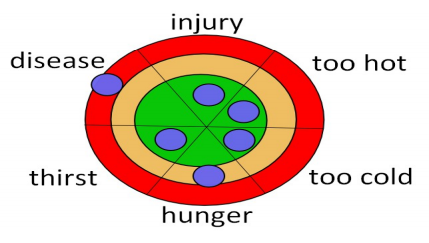
\includegraphics[width=12cm]{/figs/fig6.png}
\caption{Core SCIM model: Individual – the six causes of death in a catastrophe.}
\end{figure}

The number of deaths resulting from each of the above causes is “contained” by vital services. In the case of excessive heat and cold, this service is provided by shelter: housing (including heating, cooling and insulation) and clothing. Hunger and thirst are solved by supplies. The risk of dying from disease and injury is reduced by the security provided by public health prevention activities, health care, police and army.

\subsubsection{Levels of provision}

The next step in applying the SCIM model to the local situation is to map at what levels elements of “infrastructure” exist that meet each of the requirements. What entities own, use, manage and maintain resources that meet each critical need?

The first level is that of the individual, followed by the household, neighborhood, city, region, country, and the international level. These levels serve only as a guide. In archipelagos the island level must be included.

For example, on the individual level, each person can make decisions to control their own body temperature if they have the right resources, changing the amount of clothing they wear and devising other strategies to keep warm enough or cool enough.

In many regions of the world, most of the food arrives from the global level through markets, transport networks and retail; only a fraction comes from the national and regional level; and rarely is that food grown at the household or individual levels. (Local production, when specialized, is largely for exports, delivering to external markets at different times of year.) Items such as cooking and refrigeration need to be included.

All 18 items are similarly reviewed, as we will see later.

\begin{figure}[h]
\centering
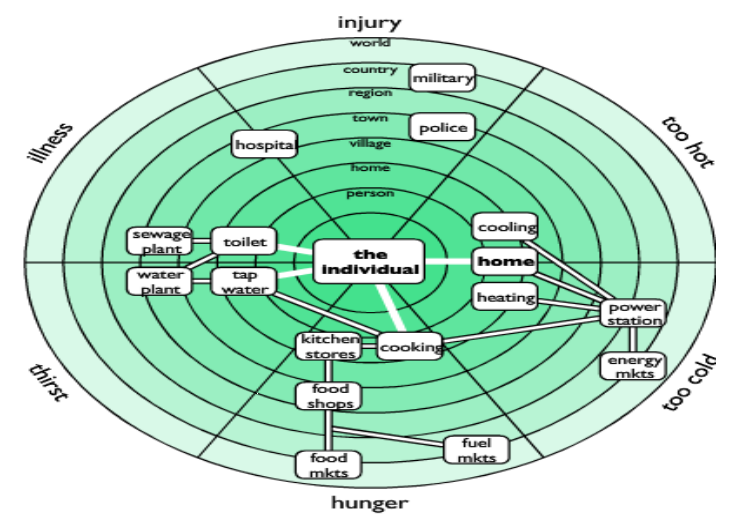
\includegraphics[width=12cm]{/figs/fig7.png}
\caption{Levels and delivery systems of the six basic needs of individuals}
\end{figure}

\subsubsection{Provision alternatives}
The SCIM model focuses attention on needs, which are generally provided by systems that work well before the crisis.

Such systems may not be substantially affected by a pandemic in a given territory. For example, excessive heat and excessive cold may not be a problem in areas where temperatures are mild, even during the most severe pandemic. In places where it rains often, thirst will most likely not be a problem. On the other hand, a number of systems at each location may be “disrupted”: they may have stopped providing needed services, they may be at risk of doing so, or the way they work may need to be changed as part of the full set of prevention and treatment strategies.

If the specific needs served by the altered system are indeed “vital” (for individuals, groups or organizations) then they will persist regardless of the system’s status. Different strategies may be used to maintain vital services:

\begin{itemize}
	\item Reduce the need (“saving” strategy). For example, use less water (or none) for certain uses, redesign systems so that some steps and ingredients are not needed, or reorganize or delegate tasks so the need for communication is reduced.
	\item Accumulate resources (“stock up” strategy). Between 2005 and 2009, many countries stocked up on antivirals and other resources. Following the 2009-10 pandemic, with many countries suffering an economic crisis, this strategy is not among the first to be considered for a threat that is not generally perceived as a priority. It goes against the motivation of convenience on the side of customers (getting products that are delivered just when they are needed, through globalized, instantaneously responsive supply networks), and also against the competitive motivations of suppliers (reduced inventories for less storage and greater flexibility)\footnote{http://www.colvet.es/modules.php?name=articulos&idwebstructure=195&idarticulo=55 Revista de Información Veterinaria, Sep 1st 2007. “A strategic food reserve for the Canaries” (in Spanish). Miguel Ángel González Cortés and Juan Manuel Santana Rodríguez.}
	\item Strengthen the system. For example, exceptional health resources can be assigned to treat influenza patients, or the transport of food can be protected. Unless resources are abundant, this strategy will require prioritizing some systems at the expense of others – delaying certain types of elective surgery until the post-peak period, for example, or even fully abandoning specific noncritical activities. In the case of staff, reinforcement strategies might include employing volunteers, recent retirees, high school seniors or students of related subjects; and providing accelerated training, cross training (so that workers train each other in a variety of basic skills), and telephone support (among experts, either from home or from other workplaces).
	\item Change the level of provision. If a need cannot be met by systems at one level, consider alternate provisioning strategies such as cultivating food locally if imports fail, importing food if local production fails, or using walkie-talkies or satellite phone if communications fail.
	\item Modify the route of delivery. For example, weekly groceries might be delivered to homes rather than fetched by shoppers from the store; liquid fuel for generators might be delivered to substitute, in the case of critical needs, for power normally supplied by the electrical grid; or therapeutic advice for certain diseases might be administered by telephone rather than in person.
\end{itemize}

\begin{figure}[h]
\centering
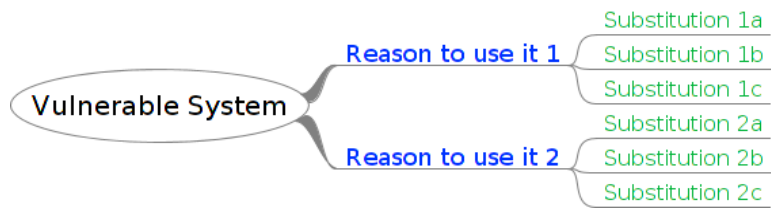
\includegraphics[width=12cm]{/figs/fig8.png}
\caption{Mind-map summary of the substitution strategy suggested in the text}
\end{figure}
\\
\\
\textbf{Alternatives: centralization / decentralization}\\
One area that deserves separate consideration is centralization / decentralization in a crisis. In industrialized countries, the last two centuries have seen the construction of highly efficient systems with a large aggregated cost but with a comparatively low cost per unit. The very complexity of these systems introduces additional risks and vulnerabilities, because each requires accurate and simultaneous operation of several subsystems in order to function. In these systems, use is decoupled from maintenance, allowing the professionalisation of their management and repair, and freeing most people from related tasks, but also creating a dependency which may become visible in a catastrophic situation.

The way out of vulnerabilities created by such complexity is usually to seek redundancy in these basic systems. In our homes, we may keep some candles for times when electricity is unavailable. Hospitals have generators adequate to operate the most vital equipment. Emergency personnel might be provided with crank or solar phone chargers.

Another possibility is to repurpose existing items. For example, if accommodation might be needed for potentially large numbers of people, standard size panels commonly used in construction may be used to rapidly build simple shelter units at a low cost per person\footnote{http://www.appropedia.org/Hexayurt}, perhaps in the context of a project for population relocation or decompression. Similarly, it is possible to manufacture water filters, stoves and toilets with resources commonly used for other purposes\footnote{ http://www.appropedia.org and http://www.akvo.org (akvopedia)}. Similar experiences exist with communication systems\footnote{http://www.wndw.net/}.

\emph{A catalog of solutions adapted to resources already available in each environment serves the same purpose as the accumulation of dedicated material.}

At a more abstract level, supplying critical needs is about making substitutions. Typically, we respond to our needs using “systems”. If a system fails, or, for lack of the supplies needed for their continued operation, a limited-use regime is entered, it is possible to use a two-step strategy: 
\begin{itemize}
	\item First, list the specific services provided by that system.
	\item Second, look for alternative ways to obtain such services.
\end{itemize}

\subsubsection{Needs of Groups}
The SCIM model goes beyond the “six ways to die” for individuals, and considers three levels of aggregation: groups, organizations and states, each of which can have their operations disrupted to the point of “death” (if they disintegrate or are otherwise unable to provide their services) because their “vital” needs are not covered.

Groups, defined as “any collection of people”, may be as few as two people. Typical groups include families, peers on a trip, or any social group. Each individual is part of a number of groups or can bind to them flexibly. 

Most groups need:
\begin{itemize}
	\item Communications (especially important for dealing with non protocolised situations)
	\item Transportation (available means of transportation, including walking)
	\item Space to meet and conduct business (such as the household for the family, a local cafe for a group of friends, and so on)
	\item Shared use of resources owned by the group (offices, telephones, vehicles and other shared items such as stoves and information)
\end{itemize}

\subsubsection{The role of groups in a crisis}
In a severe crisis, family groups and groups of people linked by activities enjoyed in common may be of particular importance. It is in these groups, defined by informal but very powerful links, where individual knowledge about the crisis and response options is articulated.

\begin{itemize}
	\item It will be families, neighbors and friends, for example, who can work out the thorny logistics of arranging child care if public health entities suggest that students should stay at home for a period of time.
	\item Neighborhood associations may in certain circumstances provide support for people who live alone, perhaps checking on them daily, monitoring their health status, and providing or seeking help on their behalf if necessary.
	\item More specialized groups such as amateur radio networks, craft clubs or groups of technologists in schools have the capacity to contribute to alternatives to some conventional services.
\end{itemize}

Therefore, the other levels can and should support this capacity to respond to crises by collecting and disseminating information and strategies that may be useful for groups.

More specifically, documents offering guidance for home treatment of less severe cases can be outlined and disseminated, along with documents to facilitate families’ and local groups’ taking part in caring for a numerically significant fraction of health-care overload in a severe pandemic. The same applies to the management of certain chronic diseases and disabilities. 

In turn, each group can make their own map of basic needs, articulate alternatives in case conventional systems fail, and see how they may contribute to the solution of common problems.

\subsubsection{Needs of organizations}
Organizations are a special kind of group with a purpose that goes beyond the combined purposes of members. Hospitals, police forces, armies and schools are all examples of organizations. An effective organization has all the needs that groups (and therefore also all individuals) have, so they must review those needs to extent that they are applicable.

In addition, organizations need three elements of what might be called “social infrastructure”, which give the organization coordination and unity of purpose, and thus allow the organization to function (“to live”) as such:

\begin{itemize}
	\item The “shared map” includes shared reality, such as what is happening, what must be done, what works and what is the correct way of doing things. During a complex catastrophe, every organization and the groups that are part of it need to know about new situations as they unfold, in order to respond by reformulating their objectives.
	\item The “shared plan” includes the activities undertaken by the various groups and individuals within the organization, often in collaboration with other groups and individuals. If the organisation's aims are reformulated, then new action plans will need to be drawn. It may be appropriate to allow peripheral units extra autonomy to redo the plans according to local situations, so that the center will not be overloaded to the point of becoming non-operational.
	\item The “shared succession model”, under non-pandemic circumstances, unfolds through recruitment or appointment and through sick-days and layoffs. In a pandemic, the availability of those involved in leadership, coordination and highly specific tasks may be affected. It is therefore necessary to anticipate who replaces the absentees.
\end{itemize}

In addition, organizations often require specialized housing and equipment to achieve their purpose. It is possible to note these needs together with the 18 generic needs. Thus, a hospital, in order to cover part of the needs of a population in terms of “disease”, has specific needs such as “sterilization”, “pain management” and others, perhaps up to a total of 50-100 items. 

It is worth keeping in mind that the SCIM model suggests that we look at “needs”, not “systems”. Thus, sterilization, which is usually performed in a hospital with an autoclave connected to the mains power supply may, in case of network failure, be performed by boiling. 

Lastly, organizations require services from other organizations. For example, a hospital may require energy, communications and police services to be available.

Each organization has its own culture and its own “vocabulary” emanating from a shared understanding of the organization's goals and methods. However, to the extent that a severe pandemic requires re-prioritizing and remodeling organizational activities, the teams in charge of forging the organization's panoramic vision can use the SCIM-OODA framework to assess conditions and transmit adjusted priorities and strategies to units within the organization so that vital services – for the whole society, for other organizations, etc – are delivered as effectively as possible.

\subsubsection{Needs of states}

Nation-states are a special form of social organization that provide services to all citizens. They provide a legal system and uphold public order, and maintain lists of their own citizens and control of their own territory.

Sometimes states also provide infrastructure services such as a national grid, ports and airports. The nation-state carries out its mission through specific organizations such as the police, army and judicial systems, which allow the state to sustain itself and provide services to citizens.

For example, the “list of citizens” is maintained at the national level with support of local entities, and territorial control is established through national sovereignty and local services such as land registries. 

Legal rules that constitute the jurisdiction are developed and implemented nationally, although there are elements which are developed and implemented locally.

So, what has been said about organizations is entirely applicable to these structures.

\subsection{OODA Loop}

Designed by Colonel John Boyd to improve the effectiveness of fighter pilots, the OODA loop involves four steps: look at what is happening (Observation); interpret the situation, imagining several likely or extreme scenarios and envisioning our choices (Orientation); determine what to do (Decision), and take the measures decided upon (Action). Following Action, Observation begins all over again. 

Updated proactively and continuously, the OODA loop uses realistic threat models to anticipate how a threatening situation is likely to develop and helps us generate agile and appropriate responses.

\begin{figure}[h]
\centering
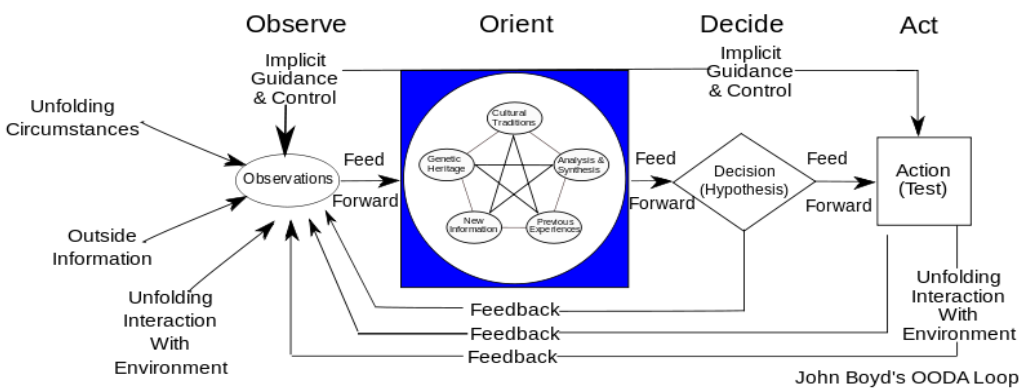
\includegraphics[width=15cm]{/figs/fig9.png}
\caption{Observation – Orientation – Decision – Action loop, John Boyd. Source: http://en.wikipedia.org/wiki/OODA_Loop.}
\end{figure}

The OODA loop items, in a crisis, are specified as follows.

\subsubsection{Observation}
In the case of an influenza pandemic, observation encompasses information about the virus, the behavior of the epidemic locally and elsewhere, the local and global response, and indicators of resilience and dependence.

Information may be fast, accurate and confirmed, but it can also be useful if it is the best possible estimate, obtained in time, and presented in an understandable way so that it is useful to make effective decisions.

In a novel and uncertain situation, we can use lists of questions, derived from our priorities and targeting both known facts (“the new virus exhibits such and such behavior”) and unknown facts (“we do not know how it will progress in the future”). As an example, see the list drawn from the point of view of public health by the European Center for Disease Control (ECDC)\footnote{http://ecdc.europa.eu/en/healthtopics/documents/0905_pandemic_influenza_known_facts_and_known_unknowns.pdf}.

The questions needed from the point of view of civil protection and the provision of essential services emerge, as we shall see, from implementing the SCIM framework. As examples, a known fact would be “we have so many cubic meters of drinking water for so many people”, and an unknown one would be “we do not know if there may be a shortage, or its possible duration”.

To answer our questions, we will use the information from external and internal news, rumors (which we must try to validate or contrast) and information systems (pre-existing or adapted to the crisis). It will be possible to use – preferably with previous tests – communication systems developed for other emergencies in recent years, based on electronic collaboration tools: wikis\footnote{http://www.crisiscamp.org/}, etherpad\footnote{http://www.etherpad.org/}, social networks (Twitter, Facebook and others), telephone networks adapted to catastrophic situations (frontlineSMS\footnote{http://www.frontlinesms.org/}) and collaborative maps (HealthMap, ushahidi\footnote{http://www.ushahidi.com/}).

\subsubsection{Orientation}
The Orientation element of the loop is about assigning meaning to what is observed, and about answering questions about what is happening, what will happen, and what we can do.

Therefore it includes having a threat model (in the case of severe pandemics, the first chapters of this document), which will be useful for the development of alternative predictive models (“how many new patients we may need to treat next week, or the week after that”\footnote{See numeric simulation annex}).

We will also need a model of available resources, so that we may consider different possibilities for action (“start a specialised hospital or not”).

Orientation is the most critical activity and sits at the center of the model, closely related to the other components. Thus, our “map of the situation” will show the areas of uncertainty which we should 

Observe more carefully and will indicate which Decisions must be made and how we might Act.

The SCIM framework is a useful tool specifically for the Orientation phase, which is a speculative non-routine activity, difficult to do in a complex crisis, at a time when there is need to prioritize and reprioritize appropriately and in a timely fashion.

\subsubsection{Decision}
Decision, in turn, refers to selecting, at the different action levels, alternatives designed to strengthen, adapt and replace pre-existing systems in order to provide essential services for the duration of the crisis.

These alternatives, as is clear from the SCIM framework, may benefit from a shared model of what the essential needs are and what levels can be positioned to address these. Once generated, these alternatives may be weighted according to their feasibility, benefits, difficulties and consequences in order to enable planners to make appropriate decisions at any given time.

\subsubsection{Action}
Actions – preferably reversible – will be taken at all levels. The primary mission of some levels will
be to facilitate, or in some cases limit, the actions of others. Levels include:
\begin{itemize}
	\item For example, at the individual level, strategies such as hand washing or actions regarding the consumption or production of resources can be encouraged.
	\item At the group level, a family or a neighborhood association may organize the care of those who are school-aged.
	\item At the town and island level, planners might procure a supply of insulin for insulin-dependent population, or train the levels they are responsible for in the strategies mentioned in this document.
	\item At the national and regional levels, entities organize services in their areas of responsibility, such as networks of hospitals and laboratories, general performance criteria, and others.
	\item On the international level, governments negotiate to deal with actions such as the production of vaccines and transnational distribution of vital supplies.
\end{itemize}

\subsection{Using SCIM and OODA}
The SCIM list of needs and the OODA loop may be used before or during the pandemic, and at any level, from individuals, families or social networks to the national or even international levels.

\subsubsection{Inter-pandemic and pandemic phases: preparedness and response}
The OODA loop and the SCIM framework can be used before a pandemic, when it is starting, and as it unfolds. In any case, the process is always about making the decisions that are appropriate at each point in order to improve the response to the direct and indirect risks on people's lives.

For example, during the interpandemic phase when this document was written, the OODA loop for pandemic response included the following steps:

\begin{itemize}
	\item On one hand, the \emph{Observation} phase included looking at the risks of influenza at the animalhuman interface, the incompleteness of the plans and preparations developed to date worldwide, and the systemic vulnerabilities that – using the SCIM framework – could be anticipated if a highly lethal and disruptive pandemic were to happen.
	\item The \emph{Orientation} phase included considering the difficulty of maintaining the intensity of preparations developed in 2005-2009, both due to what is now called “pandemic fatigue” and to the intensification of other priorities (economic, ecological, climate, and others).
	\item The \emph{Decision} and \emph{Action} phases both focused on the practical realization of two elements: a possibilistic and improvable document that could be shared through publication, and an educational program aimed at first at civil defense and essential services staff. Work done might eventually be useful (depending on motivation and resources) to draw or improve specific plans for each SCIM item, with the idea of contributing to the initiatives already developed by national and international institutions.
	\item All the above would of course be reassessed in a new iteration of the OODA loop, depending on changes in the pandemic threat, the development of plans and preparations, and other factors.
\end{itemize}

\subsubsection{Government levels: vulnerabilities}
Each level of government (country, region, island, municipality) can use SCIM with the OODA loop to do a general iteration and gain an overview of the territory for which it has responsibility. This iteration may take the form of an Integrated Needs Analytical Map (INAM)\footnote{Integrated Needs Analysis Matrix. See pages 10-11 http://resiliencemaps.org/files/Dealing_in_Security.July2010.en.pdf}, to serve as a basis for discussion of the vulnerabilities in the territory considered.

What we do is review each of the 18 SCIM items and assess whether the needs are adequately covered against the challenge under consideration, in this case a severe pandemic. For those items that are not adequately covered, appropriate action is carried out to reinforce, supplement or modify the elements of the map.

The appropriate level of government can delegate each SCIM element to the appropriate combinations of governmental and nongovernmental organizations, with the help of groups and individuals as may be needed. They can also offer their resources to the whole of society.

Specific response plans can be created that are centered not on the cause (a pandemic, a volcano, or others) but on the effect (for instance, plans for the shortage of water, food, medicines). Such planning for all hazards will complement pandemic-specific response plans. These plans could refer, in the case of shortages, to parameters such as intensity (percentage of food that stops coming) and duration (number of weeks the shortage lasts).

\begin{figure}[h]
\centering
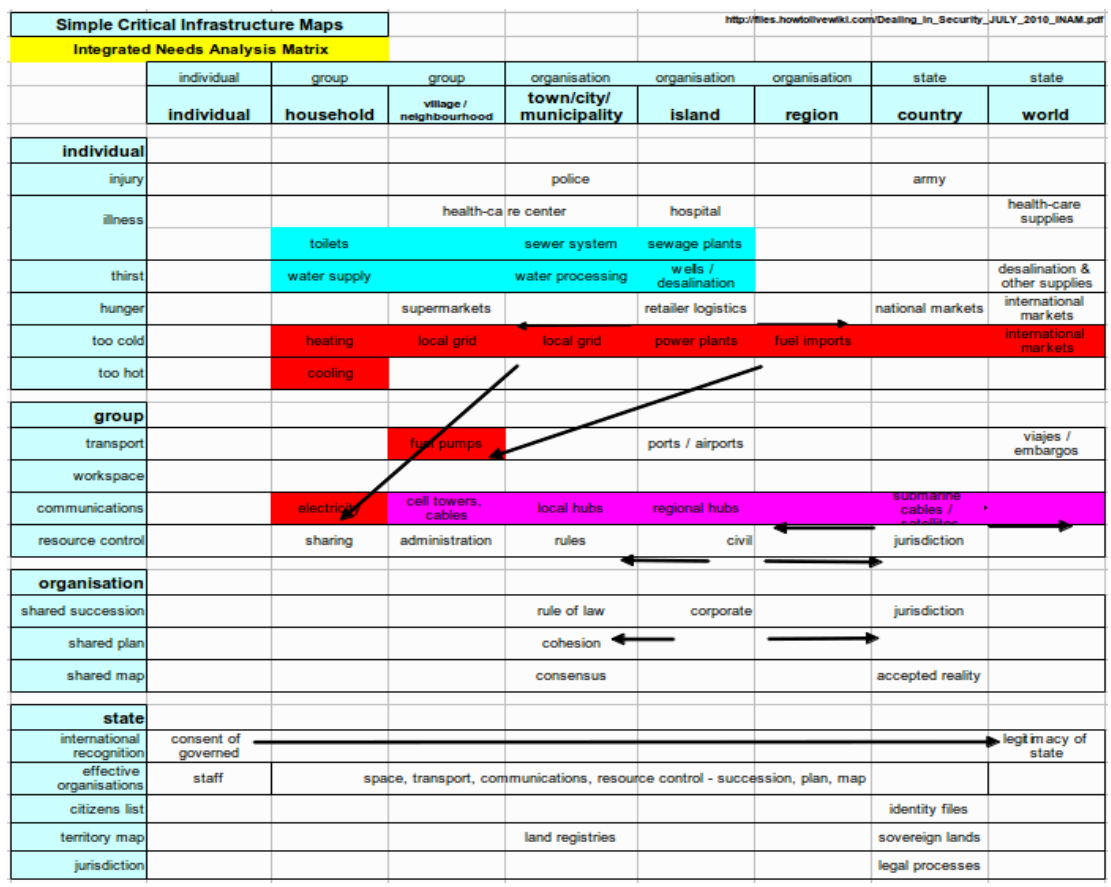
\includegraphics[width=15cm]{/figs/fig10.png}
\caption{Integrated Needs Analytic Matrix. Overview of needs and entities that cover them, for a Macaronesian island.}
\end{figure}

\subsubsection{Among organizations: interdependencies}
For each SCIM item, organizations with responsibilities in that particular area may come together to use the strategies suggested in this paper to organize information, possible points of failure and actions.

This use of OODA-SCIM between organizations is arguably the most important, since it allows direct, collaborative focus on priorities and interdependencies.

If it is not possible to cover needs through the organizations that are locally active, different strategies may be developed: local organizations may ask for assistance from organizations in other levels, and they may innovate (or copy and disseminate innovations) so that the same essential services can be delivered using other levels of execution or other means of delivery.

This way, SCIM becomes a common language that streamlines communication priorities through the “noise” of a complex and potentially chaotic situation. In this sense, SCIM resembles idiomatic subsets used for communication between amateur radio, airplane pilots, and the like\footnote{http://en.wikipedia.org/wiki/Seaspeak is an example of reduced vocabulary used to facilitate communication among people who speak different languages in specific situations.}.
\newpage
\section{RESPONSE TO A SEVERE PANDEMIC}
While the crisis is anticipated, or as it unfolds, activities are developed at all times to reduce infections, treat the sick, and maintain vital services and supplies – aiming for those three goals in combination, in the context of a severe and evolving pandemic. Activities targeted to achieve these three objectives are implemented simultaneously, and are
presented separately only for expository clarity.

\subsection{Scenarios and information}
Each level may draw their own map of the situation, with numerical and qualitative scenarios which will be based on the currently available information.
\subsubsection{Numerical scenarios: simulated waves}
Before a pandemic, or even before each epidemic wave, it is not possible to accurately predict its development, as its contagiousness and clinical severity are not known.

However, it is both possible and useful to do several simulations – not forecasts – to get an idea of the range of possible scenarios. Such simulations help in the task of organizing with flexibility, more or less in advance, the provision of resources and changes in how services are run.

To perform these simulations, computer programs such as FluAid, FluSurge, Community Flu and others have been created\footnote{http://www.cdc.gov/flu/pandemic-resources/}. Several of these programs are relatively complex, take into account the age distribution of the population and provide disaggregated figures. Others have more specific uses.

FluWorkLoss, for example, helps planners estimate worker absenteeism in various scenarios\footnote{http://espanol.cdc.gov/enes/flu/tools/fluworkloss/}.

In the corresponding annex the use of a simple spreadsheet is suggested, in which the user can type the reference population, the percentage of the population that falls sick, and the percentage of patients who die, in order to obtain values for each week of an epidemic wave. The spreadsheet plots two versions of epidemic waves, each differently useful. The first (a “fast” wave) is a local wave impacting a limited population. The second, geographically broader wave is the sum of several local nonsynchronous waves. Because it is summative and because local waves hit at different times, it graphs as a “slow” wave by comparison to any local experience. The values obtained for each type of wave are the simulated number of \emph{cases, severe cases} and \emph{deaths} for each week.

(It should be noted that a wave's duration can be lengthened to the extent that contagion-reduction measures are successful\footnote{http://www.pnas.org/content/104/18/7582.full Public health interventions and epidemic intensity during the 1918 influenza pandemic. Richard J. Hatchett, Carter E. Mecher, Marc Lipsitch.}, because, according to history and mathematical models, the frequency of cases may rise again if measures are lifted too soon.)

Conducting simulations with different values enables planners to draw qualitative conclusions, relatively constant over a range of possibilities, about the degree of monitoring necessary to detect early cases. Simulations also help to generate estimates of important time intervals, such as the amount of time that passes since the first cases are detected until their number exceeds the capacity of the health care system in its normal operating regime.

\begin{figure}[h]
\centering
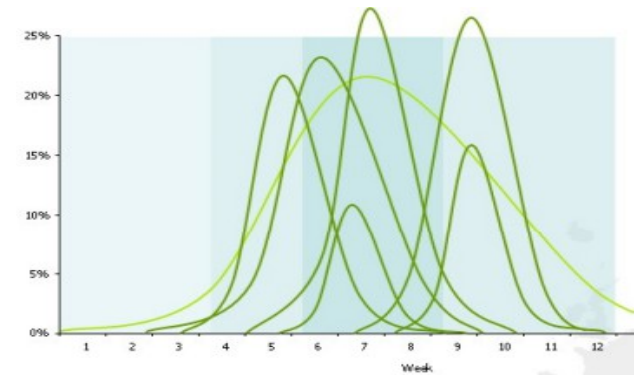
\includegraphics[width=12cm]{/figs/fig11.png}
\caption{The wave for each wide territory is the sum of smaller waves for the smaller territories that are included in it. In each part of the territory, the wave is narrower and steeper. Source: ECDC}
\end{figure}

\subsubsection{Qualitative Scenarios: Integrated Needs Map}
For each territory, especially the larger ones (country, region, island), an integrated map of needs can be drawn, listing the 18 needs and 7 levels of the SCIM model, and including, to the extent that is useful, organizations (each in its own column) that provide vital services. An example is included in the accompanying spreadsheet.

This overview will allow planners to quickly identify what needs are at risk in a given situation and place, to focus efforts on those areas. For example, there are archipelagos with particularly dry islands where “thirst” should have special consideration.

Besides anticipating potential figures pertaining to influenza cases, we may collect more or less approximate figures, based on the expertise of local clinicians, regarding pre-existing conditions and groups with particular vulnerabilities (medical, social, language-related, and infrastructure-related – see SCIM-individuals).

\subsubsection{Epidemiological and virological information}
Scenarios can be updated with objective knowledge of the highest possible quality about the reality of the epidemic in terms of illness, severe illness, and deaths – all broken down by age and presence of preexisting disease or other risk factors. 

This continuously updated information on the epidemic and the circulating virus will stream from monitoring activities carried out at different levels:

\begin{itemize}
	\item National, continental or global epidemiological and virological surveillance: WHO, ECDC, SVGE, Portugal and other countries cooperating with gripenet.pt, ProMEDmail, GPHIN, HealthMap and others.
	\item Already existing systems of epidemiological and virological surveillance at the local level, suitably adapted to a severe pandemic: primary care networks (based on all practitioners or on a sample of voluntary notifiers), hospital, and virology laboratories.
	\item Epidemiological and clinical research – for example, it is possible to obtain, before the pandemic or rapidly at the beginning, information about the usefulness of generic drugs for the treatment of pandemic influenza. It will be helpful to plan ahead how such studies may be conducted, so that they may be carried out quickly and efficiently in case of need.
\end{itemize}

\subsection{Infections reduction}
In a pandemic, most of the population is susceptible to the new virus. If the severity of the virus is medium or high, the number of patients and the proportion of patients with serious disease will overload both the healthcare system (in parallel with the epidemic waves), and the whole of society (according to the degree of disruption).

Therefore, a primary objective for confronting each epidemic wave would be to delay the peak, reduce its maximum amplitude and, if possible, reduce its volume (i.e., the total number of cases). This will attempt to reduce the pressure, both on the health system and in the wider society, and to gain time while the availability of treatments and vaccines is accelerated.

\begin{figure}[h]
\centering
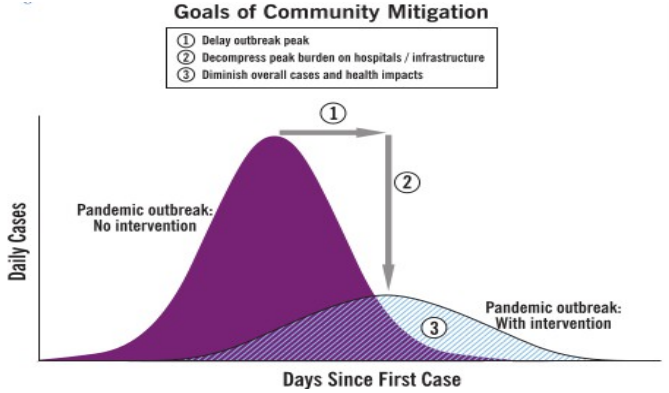
\includegraphics[width=12cm]{/figs/fig12.png}
\caption{Goals of interventions aimed at reducing pandemic “explosiveness”: delay, decrease the peak, possibly reduce the total number of infected people. Source: http://flu.gov/professional/community/commitigation.html.}
\end{figure}

A pandemic wave will be more or less rapid and intense as a function of the speed with which infections occur. A parameter representing this speed is the “basic reproductive number” or R0 (“Rzero”), which is the average number of secondary cases resulting from any one case. Simply put, if, for example, each case generates on average two cases (R0 = 2), the number of cases will grow approximately like this: 1 → 2 → 4 → 8, and so on. With R0 = 3, the number of cases would grow like this: 1 → 3 → 9 → 27, and so on.

During the 1918-19 pandemic, R0 ranged between 2 and 3\footnote{Mills CE, Robins JM, Lipsitch M (2004). “Transmissibility of 1918 pandemic influenza”. Nature 432 (7019): 904–6}. This figure is an average and depends not only on the intrinsic characteristics of the virus but also, very importantly, on human activities. As an average, R0 ultimately reflects factors such as the combination of very low propagation environments (people living basically alone) with very high propagation environments (schools, shopping centers, mass transportation, work or recreational venues, and the like).

Even if the average number of secondary cases caused by a particular pandemic influenza virus (as opposed to other diseases) may not be very high, influenza is characteristically contagious from its early stages; therefore time required for cases to multiply is short (a few days). Cases multiply quickly. If the time between generations of cases (in other words, the time between the moment of infection of a given case and the time of infection of his/her secondary cases) is about three days, 10 generations of cases will occur in a month.

For reference, we can take the wave used as a possible scenario for the UK at the start of the 2009-10 pandemic. For this scenario it was assumed that 30\% of the population would experience flu symptoms at some time during the whole wave, and that 6.5\% of the population would have symptoms at the peak week (local planning should use figures between 4.5\% and 8\%)\footnote{https://www.ncbi.nlm.nih.gov/books/NBK143060/}.

Tools to reach the above stated aim – by giving information, coordinating and facilitating society's actions – are detailed later.

\begin{mdframed}[leftmargin=10pt,rightmargin=10pt]
\begin{itemize}
	\item Influenza is transmitted at the onset of symptoms, to a lesser extent before symptoms begin, and also by way of infected people without symptoms. For maximum preventive effect, multiple measures, each partially effective, must be “stacked”.
	\item Reducing the number of respiratory contacts – such as by sending students home early for a sustained length of time – is essential in a severe pandemic.
	\item Various types of face-masks, respiratory and hand hygiene, together with other strategies, reduce the rate at which new infections occur.
	\item Given current technology, vaccines will not be available until several months after the start of the pandemic, and in smaller quantities than are needed globally. In any case it would be necessary to prepare for the orderly distribution and administration of those limited quantities of vaccine.
\end{itemize}
\end{mdframed}

\subsubsection{Imperfect layers and the time factor}
Because influenza is most contagious in the early stages of the disease, rapidly multiplying the number of cases, its spread is difficult to control. Since some of those infected may remain asymptomatic, their role in spreading the virus may prove important\footnote{Non pharmacological measures to respond to an influenza pandemic – Annexe XIII of the national (Spain) plan of preparedness and response to an influenza pandemic. Sept 2007. http://www.msc.es/ciudadanos/enfLesiones/enfTransmisibles/docs/AnexoXIII_MedidasNoFarm.pdf}.

Despite these challenges, a variety of measures can help, if used in concert, to slow the pace of an epidemic wave. These measures have different usefulness:

\begin{itemize}
	\item Border closure has been suggested but is not generally considered a viable strategy. Mathematical models indicate that even a reduction of more than 95\% of human movement across borders (which would be both highly disruptive and difficult to establish since borders are, after all, porous) would delay the entry of the virus by only a couple of weeks. Once there are cases inside the borders, the strategy – if it has been used – should be abandoned. During the pandemic of 2009-10, the international spread of cases began during the first few weeks and probably before the situation was first detected.
	\item Isolation of cases and quarantine of contacts (see below, 2.b) are important, but by themselves are not able to contain the spread of the epidemic, for the reasons given above.
	\item Social distancing – or, more acurately, reduction in the number of respiratory contacts. This includes restricting international and domestic travel (already mentioned) and, above all, measures taken at school, at work and within communities (see below, 2.c).
	\item Personal protective measures such as respiratory hygiene, hand washing and face-masks (see below, 2.d) also constitute an imperfect barrier to the spread of the virus.
	\item Vaccines, which will not be available in the first stages given that it is not possible to know in advance which virus will cause the pandemic. Distribution and administration must be prepared for (see below, 2.e).
\end{itemize}

While none of these mitigation measures, applied by themselves, will be able to achieve the desired goals, both history and numerical simulations make it clear that their combination can achieve a significant mitigating effect, slowing the spread of the virus through human communities. Those same studies show how important it is that the measures are applied early (preferably before the epidemic starts its accelerated ascent) and maintained over time because, if the measures are withdrawn too soon, the epidemic wave rises again.

In this sense, it is expected that public motivation to implement the proposed measures will vary depending on the perceived severity of the pandemic, the disruptive effects of the measures themselves, and the length of time for which they need to be maintained. Therefore, updated information on the situation should be regularly collected, effectively disseminated and clearly communicated so that all involved in applying mitigation measures understand both the “whys” and the “hows” of carrying them out and, further, the number of weeks they may be needed.

\subsubsection{Isolation and quarantine}
Isolation involves separating symptomatic individuals from others and restricting movement and activities in order to prevent transmission of infection to others. It applies to ill individuals during the duration of symptoms, i.e. about 7-10 days from the first symptoms. It is considered useful over the entire epidemic wave. Non-severe cases can implement isolation at home or in specifically designated and prepared locations.

Like isolation, quarantine involves separating people and restricting movement and activities, but it applies to those who have have been exposed to the virus through contact with an infected person. It lasts from the time of exposure through the incubation period, after which the individual will have shown symptoms or not. The precise number of days will be adjusted according what is known about the period of incubation for the pandemic virus. In contrast to isolation (which is thought to be useful throughout the pandemic), quarantine may not be practical in times when many people are sick simultaneously. 

Quarantine may be implemented both at home and in specifically designated and prepared locations.

Activities to facilitate implementation may include the following:

\begin{itemize}
	\item Disseminating information and instructions from Public Health, and centralizing reports on the difficulties and innovations in their application in order to redesign strategies and make them more powerful and easier to perform.
	\item Enhancing mutual-aid networks of family, friends, neighbors, coworkers, and others. Proposals may be put forward so that every family, building or street, group or network of people, may make a list of people and their contact information so that all can be contacted at least daily to confirm their health status and supported with SCIM-individual and SCIM-group needs (food, medication for the flu and other illnesses they may have, communication, and other needs) in order to facilitate their stay in the place of isolation or quarantine. Mutual support will be particularly relevant for people who live alone and for households with one or more dependents. 
	\item Organizing places for isolation or quarantine and assembling resources needed to serve for several days, at least with camping-site comfort levels. (Again, SCIM-individual and SCIMgroup.) This strategy may be of interest in two specific cases:
\begin{itemize}
	\item First, quarantine can serve health-care workers who are most exposed to influenza cases. Frontline health-care workers themselves have suggested the option of a work schedule comprising several days of work during which they do not return to their homes, followed by a period of quarantine, followed by a family visit, and then a new shift of work away from home.
	\item This strategy may also be considered as part of the extreme reduction of respiratory contacts for people who deal with infrastructure elements that are both vital and highly specialized (such as power plants technicians).
\end{itemize}
\end{itemize}

\subsubsection{Reduction of respiratory contacts}
Infectivity depends partly on characteristics of the virus (higher or lower adaptability to human cells, for example) and cannot be controlled. However, “intrinsic infectivity” being equal, reducing the number of respiratory contacts among different people in a given time will result in fewer opportunities for infecting and being infected, and therefore in a reduction of the multiplication coefficient.

In fact, both analysis of the experience of the 1918-19 pandemic\footnote{ http://www.nih.gov/news/pr/apr2007/niaid-02b.htm on how measures were applied differently in two American cities, and how the epidemic wave differed between them.} and numerical simulation studies show that reducing respiratory contact has an important effect on the shape and volume of the epidemic wave.

In particular, and this is very important, these measures effectively reduce mortality only when implemented early on, that is, when only a tiny percentage of the population has fallen sick\footnote{Public health interventions and epidemic intensity during the 1918 influenza pandemic. Richard J Hatchett, Carter E. Mecher, Marc Lipsitch. http://www.pnas.org/content/103/18/7582.full}. Pandemics are like forest fires, which are more controllable if we act while the fire is small. Because inevitable delays in diagnosis and organizational difficulties are to be expected in a severe pandemic situation, taking a risky “watch and wait” approach means missing an opportunity to mitigate a worst-case version of a pandemic. By contrast, erring on the side of caution by initiating action sooner rather than later is likely the only way to avoid having acted too late. Furthermore, if it turns out that contact reduction measures will not be needed after all, they can be reversed, whereas there is no reversing an explosive pandemic wave. 

Strategies to reduce respiratory contacts, and actions to facilitate the implementation of those strategies follow:

Keeping students at home early and in a sustained manner. The social costs of this measure make its applicability low or inconclusive in mild pandemics, but no-one doubts its usefulness in a severe pandemic. In a severe scenario, keeping children home becomes a critical tool for curbing the speed at which infection spreads: schools are, after all, crowded places where respiratory contact density is very high, and influenza is especially infective among the young. Early and sustained implementation reduces infections in young people, in their families, and among family members' contacts in other environments. Thus it serves to protect the whole of society.

For ease of implementation, the following guidelines are helpful:

\begin{itemize}
	\item The motivation and rationale for these measures should be disseminated: the goal (to help minimize accelerated multiplication of the disease), the biology of the transmission (at the beginning of the disease, even before symptoms) and the limitations of other strategies (masks).
	\item The “custody function” of schools should be fulfilled through the facilitation of social selforganization and the detection of disadvantaged groups in need of additional support. Children need to be cared for by adults in small and stable groups, thereby reducing the number of breathing contacts per person.
	\item The “nutritional function” of schools – particularly important for those students who depend on school meals: both parents work away from home, poverty, distance between school and home – may be delivered making use of school kitchens to provide cooked meals (either by asynchronous transfer or the use of mini-dining halls with only a few students in each classroom), even if there are no lessons.
	\item The “learning function” of schools can be carried out remotely, with distribution of materials from time to time and in a staggered fashion, using radio and television, with training given at home by older students to younger students or among the same age group, among other strategies.
	\item The possibility of organizing small, very stable multi-family groups has been suggested. An adaptable model might consist of 3 families of 4 people each (2 adults and 2 children). They could create a first group of 2 adults and 6 children, who would stay in the larger home; and a second group of 4 adults who would live in one of the two other homes, go out with protection and take care of bringing in supplies for the adults and children sheltering in place. This arrangement, presumably, would maintain a certain “sustainable normalcy” while decreasing the key variable: the number of different people each person – and particularly the most vulnerable and contagious – establishes respiratory contact with.
\end{itemize}

In the workplace, suggested options include working from home when possible, flexible scheduling to reduce the number of people in the workplace, cross training (in which each worker learns to perform the essential functions performed by other workers, to reduce the need for all being present), and performing asynchronous transfer of objects (leave the object in a place, where it is picked up by the other person later) in order to reduce respiratory contact.

Health-care work is a special case and, as discussed below, requires separate places and circuits for people with different probabilities of being infected, and in some cases the setting up of see-through barriers using available materials.

As for transport of people, the recommendation is to avoid public transport when possible, perhaps replacing it with private vehicles used by a limited and stable number of people, again in an attempt to reduce the number of respiratory contacts each person encounters. The use of staggered working hours can further reduce public transport congestion

For transport of goods, asynchronous transfer may be used, reducing the number of respiratory contacts workers encounter when loading and unloading.

The clustering of people in food markets can be reduced using several simultaneous strategies: aggregating several days’ worth of shopping, having one shopper shop for more than one family, arranging home delivery, or expanding open hours to reduce the number of people simultaneously using each location. In an extremely deadly pandemic, home delivery with respiratory protection for people working in the supply chain could become an important strategy. Prepositioning supplies where people are (“cattle to town”) has been suggested as an idea for an extreme pandemic.

In a highly lethal pandemic, public health recommendations would certainly include avoiding (and discouraging) public gatherings, from the beginning of the epidemic wave.

Finally, historical experience demonstrates that, when life-threatening epidemics (especially those spread through respiratory contact) strike cities, a measure of “urban decompression” takes place. Intent on avoiding infection, a certain percentage of the population will muster the means to leave the urban environment and settle in the countryside for a time. This strategy, which may be more or less feasible in terms of the living conditions of a particular rural environment, may raise logistical difficulties in ensuring adequate supply, communications and other basic needs. These challenges can be explored systematically with the SCIM-OODA tools. Solutions may require the use of distributed infrastructure of the sort used in refugee camps and for development\footnote{http://www.akvo.org/wiki/index.php/Main_Page and http://www.appropedia.org}, albeit at a much larger scale of “respiratory decompression”.

\subsubsection{Barriers, hygiene and other containment measures}
Barriers to ready transmission of the virus, although these are not normally regarded as effective if implemented on their own, can contribute along with the other measures.

As for commercial masks, there are three basic types: surgical masks, FFP2 filtered and FFP3 filtered (labeled N95 and N99 in the United States); then there are the washable cloth masks.

Important features for all face masks include, of course, how well they filter air at the mouth and nose as the wearer breathes inward (assuming the wearer the carrier is healthy) or outward (assuming the wearer is sick). Also important is how well the mask can be fitted to the face, leaving no gaps.

All must be used appropriately\footnote{http://www.msc.es/ciudadanos/enfLesiones/enfTransmisibles/docs/AnexoXIII_MedidasNoFarm.pdf}.

\begin{itemize}
	\item During the 2009-10 pandemic, use of surgical masks was recommended for cases and contacts (to prevent “outward” spread from them to healthy people around them), and for healthcare workers exposed to continuous and close contact with the public (1 meter or less). Subsequent studies have shown that their usefulness increases if passage of air through the edges of the mask is avoided.
	\item The use of FFP2 masks was recommended for healthcare workers exposed to respiratory patients. Its use is limited to a few hours, and not recommended for reuse. They must be adapted to the face following precise instructions. Its availability would probably be very limited at the population level. 
	\item The use of FFP3 masks – with limitations similar to FFP2, and more expensive – was suggested for use by medical staff performing aerosol generating procedures.
	\item A fourth type of face-mask can be made from washable fabric, say a cotton t-shirt, which is boiled in water for 10 minutes and then cut and sewn as a mask, with several layers of tissue for the mouth and nose and good lateral closing\footnote{Dato VM, Hostler D, Hahn ME. Simple respiratory mask [letter]. Emerg Infect Dis. 2006 Jun. http://dx.doi.org/10.3201/eid1206.05146 http://wwwnc.cdc.gov/eid/article/12/6/05-1468_article.htm}. These masks have an advantage in their potential for widespread use, as they can be manufactured on a large scale in the community or even in the home. They have not been thoroughly evaluated, and their effectiveness would differ depending on the quality of manufacturing and how they are used, but would likely be used in the absence of sufficient resources in a severe pandemic.
\end{itemize}

Overall, the danger with masks is that they may be – wrongly – seen as a substitute for other measures. They should be considered a supplement when other measures cannot be applied in full force, as will be the case with essential jobs that must be performed in spite of a pandemic situation, and where close contact with patients is inevitable, either in a health-care situation or, for example, in caring for the sick at home.

With regard to hygiene, three practices are recommended: respiratory hygiene, hand washing and cleaning of surfaces:
\begin{itemize}
	\item Respiratory hygiene refers to cultivating habits designed to avoid propelling large amounts of virus into the air and to avoid depositing them on surfaces. People should cover their mouths and noses when they cough or sneeze, coughing into the crook of their elbows. They should use paper tissues to receive respiratory secretions, dispose of these after use in close-by bins, and perform hand hygiene after coughing, sneezing or after using tissues.
	\item Washing hands meticulously with soap and water or with alcohol-based products should be done several times a day, especially after coughing, sneezing or being exposed to secretions from influenza patients. The recommended procedure is as follows: wet hands with water; apply soap and rub hands together for at least 15 seconds, cleaning between fingers and under fingernails; rinse with water; dry hands with a disposable towel; and turn off the tap with that towel. Devices such as the Tippy Tap\footnote{http://www.akvo.org/wiki/index.php/Tippy_Tap and http://www.tippytap.org/} or appropriate adaptations might be used, as they are simultaneously hygienic and low cost, and could therefore be as ubiquitous as needed.
	\item Cleaning surfaces (perhaps with a dilute bleach solution) is also part of the hygienic recommendations.
\end{itemize}

Among other containment measures, the use of see-through barriers, similar to those used in banks and chemists between the worker and the customer, may be considered for particular situations (say, for transport drivers).

Furthermore, ultraviolet light, or a combination of temperature and high humidity\footnote{ http://www.ncbi.nlm.nih.gov/pubmed/21731764 PLoS One. 2011;6(6):e21481. Epub 2011 Jun 24. Dynamics of airborne influenza A viruses indoors and dependence on humidity. Yang W, Marr LC.} (see research with animal models\footnote{http://www.plospathogens.org/article/info:doi/10.1371/journal.ppat.0030151}), might be useful in reducing secondary infections in certain environments and locations – maybe with a powerful effect if those locations contribute importantly to spread.

To facilitate the above measures, the following activities may be undertaken:

\begin{itemize}
	\item Deliver and explain the information to the public, if possible before the local epidemic wave starts. Use electronic means where feasible, and also physical posters and reminders.
	\item Organize the availability of hand-washing stations (either pre-existing customary ones or those manufactured for the occasion) with soap and water.
	\item Check locations where it may make sense to have see-through barriers made from available and appropriate materials, taking care to maintain adequate ventilation.
\end{itemize}

\subsubsection{Vaccines}
Organize the distribution of available masks and facilitate the manufacture of cloth masks. 

Remind users that masks are not a substitute for respiratory contact reduction.

Vaccines are an important tool when available in sufficient quantity and on time. Therefore, the production of an abundant and reliable vaccine sufficiently tailored to the pandemic virus certainly constitutes a priority in a severe pandemic.

However, the experience of previous pandemics, including 2009-10, suggests that – until new vaccine technologies can be developed, far superior to those currently used to produce seasonal influenza vaccines – production will probably be insufficient relative to demand, and even the first dose will be delayed several months from the start of the pandemic.

Alternatives for producing greater quantities of vaccine in shorter times are being developed. It is anticipated, however, that it may take years for them to be available, and there is no guarantee that the efforts underway will bear fruit.

Therefore, and especially in the first months of a severe pandemic, attention should be focused on the rest of the strategies.

Once a vaccine is available, decisions must be made about which population groups will be vaccinated first, given that quantities of vaccine, at least initially, will likely be limited. This decision is, in general, made at the national level, where priorities will be assessed based on scientific information of the highest quality, gathered and analyzed right up until the date vaccination begins. In a situation of seasonal flu or mild pandemic, the priority is to protect those who are vulnerable to complications. In a severe pandemic situation, the priority would be most likely to protect the most essential workers, which would in turn protect the rest by maintaining vital services.

In any case, the following groundwork will be need to be facilitated:
\begin{itemize}
	\item Gathering and centralising information about the specific number of people in each target group.
	\item The vaccination process itself, including the distribution of scientific information about the effects of the vaccine and the centralization of information about possible incidents and side effects.
\end{itemize}

\subsection{Caring for the ill}
During a severe influenza pandemic, the number of patients, hospitalisations and deaths may be high. Simultaneously, other illnesses, accidents, births, and all the other health issues health-care services are needed for will continue to exist.

The goal is to facilitate in all areas – hospitals, primary care centers and homes – such that treatment, appropriate in terms of real resources, can be administered, while reducing infections in these environments.

It will also be necessary to organize the transport of people and material resources. Attention should be paid to the provision of supplies and services for healthcare facilities and medical transport, again simultaneously trying to minimize infections in these environments.

The provision of essential medicines may be affected by the disruptions a pandemic is likely to cause. It is also possible to obtain, before the pandemic or rapidly at the beginning of it, information about the usefulness of generic drugs for the treatment of pandemic influenza.

This aim requires adaptations, which may be substantial, not only in terms of resources but also in the way the provision of these services is facilitated. These adaptations – which we will see in detail in the following subsections – include organizing healthcare in the network of centers; preparing reporting mechanisms, patient selection and transport; developing and reworking plans for each primary care center and hospital; and preparing epidemiological information circuits.

We must take into account the differences between a normal situation and a severe pandemic:

\begin{itemize}
	\item First, there are resources that become more limited: for example, staff may be ill (or taking care of ill relatives) at home, and material resources may become scarce.
	\item Second, precisely because of the exceptional situation, some resources can be made more readily available than they normally would be otherwise: people who stay in their homes and are able to help their families and neighbours, premises and vehicles that are released totally or in part for medical use, people who are “probably immune” after having been ill, and others.
	\item Finally, attention should be paid to site-specific resources or circumstances, either from the physical environment (such as microclimates), from the social environment (such as communities with different languages), or others that may somehow condition health-related activities.
\end{itemize}

Civil protection services and essential services may act to facilitate adaptations in information and transportation systems, and in primary care and hospital care, in two ways:
\begin{itemize}
	\item Supporting health-care workers in their planning activities. Each center’s plans may be developed and improved in a short time from open templates, which can be shared publicly except for hospital-specific data such as names and personal contact information, or location of “sensitive” devices and resources. Each template would include the aims and methods, and room for specific data. The annexes have samples (shared under an open license, as is the whole document) to facilitate their use, circulation and incremental improvement by all stakeholders.
	\item Providing space and resources of all kinds, such as communications, transport for health-care workers visiting patients in their homes, or accommodations for health-care workers for whom it is preferable to spend a period in quarantine after being exposed to ill patients and before going home.
\end{itemize}

\subsubsection{General organization of health-care}
In a severe pandemic, as opposed to a localized disaster, the overload in health care will be similar in magnitude in neighbouring territories\footnote{“Neighbour” is defined here not only in terms of proximity but also in the sense of population flow, as in an instance where a certain region A has more interchange of people with the physically more distant region B than with the physically closer region C.}, and demands and disruption will be simultaneous too. 

Therefore, although the plans and methods can and should be shared and integrated, the emphasis will be on using human and material resources that are available locally. (The definition of what “local” means should be adapted to each resource.)

Each territory and each health-care center should create and update their action plans. The plans for each territory and each center would include at least the following elements:
\begin{itemize}
	\item Dimensioning of needs. Scenarios will be prepared based on different levels of infectivity and severity. Information (or estimates) will be collected on vulnerable or special-needs populations: people living alone, dependent, insulin-dependent diabetics and others.
	\item Reduction of respiratory contacts (staff, patients and families). Health care facilities must organize differentiated access points and circuits for patients with and without respiratory symptoms or fever, arrange proper use of barriers and cleaning, and organize phone support where possible (for certain diseases, in the case of doctors with risk factors, and similar situations).
	\item Management of human resources. It must be taken into account that, as a wave pandemic progresses, the number of people who need care will rise as the number of available health-care workers will be reduced. Local listings – of unemployed health-care workers, recent retirees and students in their final year – can be set up for substitutions (replacement of a worker who's ill), reinforcement (more staff needed for more patients) and volunteering. Accelerated training can be organised for the diagnosis and treatment of influenza and, where applicable, other common diseases. The possibility of counting on the “probably immune” (people who, having overcome the disease, are able to contribute, and whose number will increase as the wave progresses) has been considered; this strategy would have appropriate limitations due “not really immune”, and also to possible confidentiality issues and risk of misuse of information.
	\item Reorganization of health-care and prevention activities. Some activities may be delayed (elective surgery, certain preventive activities) and others may be distributed in space (outpatient clinics moved to larger buildings or even outdoors), or done by telephone or through see-through barriers.
	\item Distributed catalog of material resources and potential “substitutions” (IV.1.c). This will include inventoried items such as respirators, infrastructure items such as communications, respiratory protection equipment, essential drugs for influenza (antiviral, antibiotics, antipyretics and generics) and for other diseases (analgesics, anti-inflammatories, anesthetics, oxygen, asepsis and sterilization, etc). 
	\item The most appropriate treatment with available resources (at home, in the community or in specialized centers) can benefit from the collection and dissemination of designs to be used in health-care (from respirators to intravenous devices) developed initially as “appropriate technology for poverty”, and which might be useful in situations where demand exceeds production and distribution capacity\footnote{http://www.appropedia.org/Portal:Medical_Devices}
\end{itemize}

\subsubsection{Citizen information and patient triage and transport}
The most advanced model of the citizen information, patient triage and patient transportation strategy is seen in 012-112 type integrated services (call centers), which are based on central services giving and collecting information via telephone and, if necessary, recommending actions or mobilizing peripheral resources such as ambulances.

In a severe pandemic, these services must be protected, enhanced, supplemented and, if necessary, revised to maintain their functionality and basic methodology:
\begin{itemize}
	\item Protection during work will include the same elements mentioned for healthcare in general: personal protective equipment, see-through barriers, distance, separate accommodation to avoid simultaneous infections, etc.
	\item These services will apply protocols that, in principle, will be an extension of those already used to manage phone calls on a daily basis: collecting data about the patient, location, symptoms and vulnerability; using a decision-making algorithm to recommend home treatment, activate home visits, recommend or activate transport to the appropriate level, and manage deaths. The protocols may be changed according to the trends of the epidemic. An analysis of a subset of the calls processed in previous days will let these services know what information citizens demand and the situation requires, so that this information can be disseminated through mass media channels.
	\item In order to complement the resources owned by the health-care system, transport will be done either with self-owned, loaned, or adapted vehicles; and appropriate recruitment strategies and accelerated training of staff will be carried out. Transportation staff must be managed (shifts, volunteering, and so on), as mentioned, along with the medical staff in general, and trained (with regard to hygiene, symptoms, personal protection and vehicle cleaning). The number of vehicles must be known, supplemented where necessary with non-health-care vehicles that can be used to transport patients and healthcare workers (for home visits), and adapted for easy cleaning between uses.
	\item Since the services mentioned may not exist in some places, or may be insufficient in others, it is desirable to supplement them with a distributed network that meets the same basic functionality. So, the mass media may be used to distribute copies of the protocols, in simplified language, so that people can solve in a distributed fashion an important percentage of the situations; this initiative will be helped by knowledge of what FAQs are needed, derived from analyzing samples of the questions received by the central systems. The network of phone contact points (eg local health centers or social-use centers) will also be broadcasted, with recommendations for their appropriate use.
\end{itemize}

\subsubsection{Primary care and home care}
In a severe pandemic, primary and home care systems are intended to provide or facilitate the best health care (therapeutic, preventive and social) that is possible under the circumstances, with the resources actually available.

To do this from the beginning of the pandemic and with the necessary changes according to the situation, primary care centers will develop plans to help them in their operations.

These plans will reflect the relevant information\footnote{This information, continuously gathered, can be considered as the “Observation” stage within the OODA loop}:
\begin{itemize}
	\item Size of cared-for population, with an idea of the distribution by age and sex, if possible.
	\item What health conditions they present, with approximate sizes of groups by disease, pregnancy status, conditions of vulnerability, and other factors.
	\item What resources are available in terms of workplace, experienced staff (including patients educated about their own illness), transport and communication resources, and other resources. 
\end{itemize}

The plans will also reflect the health-care organization of that particular center (see section 3.a), using outlined architect plans as appropriate to describe the center zoning, and coordination with information systems and transport (section 3.b) and hospital (section 3.d). 

Many mild cases (such as occur with seasonal flu), and a portion of the severe ones if hospitals cannot cope with demand, will require treatment and support at home. The Pandemic Influenza Preparation and Response: A Citizen's Guide, edited by InSTEDD in 2007\footnote{https://instedd.org/blog/instedd-citizens-guide-to-pandemic-influenza-the-flu-manual/}, provides in Chapter 3 guidelines for handling different situations. Other sources can also be reviewed\footnote{https://www.mayoclinic.org/diseases-conditions/flu/diagnosis-treatment/drc-20351725}. Home treatment will need support to be facilitated as much as possible:

\begin{itemize}
	\item Provide training (perhaps using the media at the start of the pandemic) on basic skills in the management of influenza (measuring vital constants, managing fever and respiratory failure) and of common diseases and injuries.
	\item Facilitate neighbors caring for neighbors (mutual assistance networks and telephone networks for certain diseases, shopping for the frail, assisting people who live alone), including notifying the healthcare system when cases or complications occur.
\end{itemize}

\subsubsection{Hospitals network}
In a severe pandemic, hospitals' goal is to provide or facilitate the optimal care that is possible under the circumstances, with the resources actually available.

Depending on the degree of expected overload (“scenarios”) hospitals may be re-conceptualized as a network of hospitals within each territory (an island, for example). To that end, a flexible organisation may be created by territorial segmentation and “specialised use” for relatively mild cases, convalescence, severe cases, and diseases other than influenza. To pre-existing resources, field hospitals may be added, either using tents owned by the military or civil protection, or built specifically for this purpose (V.4.a and V.4.f).
From the beginning of the pandemic, and as situations change, hospitals will need to develop plans to help them in their operations.

Such plans will reflect relevant information:

\begin{itemize}
	\item Contact data for people inside and outside the hospital (“coordination”). Such data should be accessible with appropriate limitations, only for those who need them.
	\item Data on cared-for population, if possible with estimates of the age-and-sex distribution and health conditions they present. Where possible, the figures are estimated by disease groups, pregnancy, vulnerable conditions, and other factors.
	\item A current inventory of available resources, including premises, technology, human resources, beds, operating rooms, dialysis units and other devices, and scientific resources (usable research capacity to assist in the quick search improved diagnostic and therapeutic elements directed to influenza and other major diseases).
\end{itemize}

The plans will also reflect the organization of each hospital, and of care in particular (see section 3.a), using simplified architectural plans as appropriate to describe the center zoning; and coordination with information and transport systems (section 3.b), primary care (section 3.c) and other network hospitals. Health-care organisation will have specific features in hospitals:
\begin{itemize}
	\item To decompress demand, it will be possible to book beds or areas of the hospital for influenza cases, to delay elective surgery, to consider hospitalisation at home and to assess the relative risk of home births.
	\item To protect the families of staff exposed to influenza, offer staff accommodations away from home for several days of quarantine prior to family visits. (This can also be done with primary care staff dedicated to caring for people with the flu.)
	\item To protect the hospital’s functionality, infrastructure needs of the hospital and available critical infrastructure replacements (IV.1.c) will be assessed.
	\item To protect the decision-making function, internal and external coordination will be reviewed with committees (including an appropriate staff substitutions chain), and contacts with organizations that provide basic services to the hospital.
\end{itemize}

\subsection{Continuity of vital services and supplies}
What’s been covered so far has to do with anticipating the damage that a severe pandemic could produce locally, and preparing and developing the necessary measures to address the epidemic itself. 

However, the analysis of the effects of the illness and death shows how a severe pandemic would impact – more or less intensely – vital services and supplies.

In anticipation of this impact, in as the crisis unfolds, a basic SCIM map for the territory of interest (country, region, island, or municipality) may be drawn. The elements of this map will assessed and solved for using the OODA loop to ensure that the main risks are covered to the extent possible. 

At a first level of coping, conventional critical infrastructure systems are strengthened so that they can continue to function as they did before the crisis, if at all possible. Thus, we’ll strive to ensure that regional power plants remain operational and that fuel supply chains continue to function. Operational continuity should be protected by protecting the people who keep critical infrastructure functioning. If conventional systems fail in a severe pandemic, a different level of coping is entered, and every need will be solved with the appropriate substitutions (IV.1.c).

Guidance is detailed below for each of the 18 SCIM items.
\subsubsection{Individuals: Excessive heat and cold}
In a severe pandemic, in regard to protection from excessive heat or cold, attention should be paid to three groups of people:
\begin{itemize}
	\item Those who usually do not have sufficient shelter, clothing, heating or cooling systems (poverty).
	\item Those who are relocated to temporary accommodations for any of several purposes: population decompression (urban residents going rural to reduce respiratory density, people in institutions being relocated when that is possible); isolation (the mildly ill); quarantine (passengers at the start of the pandemic, health-care personnel before they return to their families, and other situations); extreme respiratory protection (essential services personnel such as those responsible for the operation of a power plant), and others.
	\item The whole population (especially vulnerable people such as children, the elderly and people with limited mobility) if the weather is extreme and fuel supply or heating and cooling devices maintenance may fail.
\end{itemize}

A variety of action alternatives should be considered, including the following:
\begin{itemize}
	\item Recommendations to the public on the use of existing available resources. In the instance of excessive heat, recommendations might include preventing solar heat gain by insulating windows when the sun hits them, seeking relatively cool spaces, wearing lightweight and breathable clothing and footwear, spritzing the body with water and resting during the heat of the day. In the case of excessive cold, recommendations should include using clothing, blankets, sleeping bags and other items, such as folded towels or crumpled paper between layers of clothing, for personal insulation; and creating warmer spaces by insulating windows and/or fashioning a small tented space inside a room to hold body heat.
	\item Using “distributed technology” (rather than grid-connected) devices: evaporative cooling, or nonelectric stoves rated for indoor use, according to safety guidelines\footnote{http://www.star-tides.net http://www.appropedia.org}.
	\item Using unoccupied dwellings or other structures such as tourist, educational, and sports centers, for possible relocation of people. Relocation may be necessary for a shorter or longer period, or only at certain times (work, leisure and so on).
	\item Rapidly constructing suitable temporary structures, using methods developed for camping, refugee camps and development\footnote{http://www.300house.com Http://www.appropedia.org/Hexayurt}. Such structures should be designed with thermal insulation and effective heating and cooling in mind.
\end{itemize}

To facilitate the implementation of these alternatives it will be useful to undertake the following activities, among others:
\begin{itemize}
	\item Prior to the crisis, gather information regarding both needs and various technical resources that can be used to meet them. Actively test methodologies so that these will be available if the need arises \footnote{As an example of such tests, there are the STAR-TIDES demonstrations. http://www.star-tides.net}.
	\item Provide information to the public. In many cases, solving for needs is about people at hand using resources that already exist near where the need arises, whether that is an individual, housing, neighborhood, or municipal need. Mere knowledge of these resources' potential usefulness and instructions on how to use them can make a difference.
	\item Provide information, connections and priorities to groups and organizations close to the people who have needs, who have the resources to assist others, or who can unlock sharable resources.
\end{itemize}

\subsubsection{Individuals: Food}
\\
\textbf{Reinforcement and modifications of the existing system}
In a severe pandemic, the ill and those who are caring for them at home will not be able to fulfill their usual workplace roles for the duration of an illness and convalescence. Moreover, people with symptoms (even if those symptoms are mild) and those who live with them may be requested to avoid respiratory contact with others. Thus they would be unable to carry out their usual responsibilities, too. Finally, there may be secondary disruptions due to failures in transport systems and self-reinforcing disruptions may occur when supply chain points of failure lead to counterproductive reactions. 

All of these factors can lead to disruptions in the food supply chain at various points: production and processing, transportation, distribution, retail, storage and cooking. By reinforcing each point in the supply chain, we contribute to ensuring the whole.

\begin{itemize}
	\item As critical personnel in a decentralized but essential system, agricultural workers, farmers and food processors will face the task of producing and processing food despite the obstacles a severe pandemic will present. Beyond strategizing to limit infection, all who have roles in the food system, from farm to table, could create networks for mutual aid in case of illness, not only for treatment of illness but also to ensure that the work of food production, processing, and distribution can continue. Cross training, ready sharing of crucial information, and involving volunteers should all be part of preparation for a pandemic. 
	\item Transport will be discussed later, but it is obvious that foods are part of the priority load even in the most severe pandemic situation.
	\item Retail distribution of food is a part of the chain in which respiratory contacts are usually frequent, and maintaining functionality while reducing infections requires organizational changes that will be different in each area. A simple element would be to reduce the number of trips to the market, by making weekly lists instead of every few days. The second basic concept is “asynchronous transfer”. A relatively conservative model would be to provide purchasers with a map of the location of food so they can plan a tour of the distribution center, reducing the length of stay and therefore the number of people present at the center simultaneously. A model with greater reduction of infections could be the use of mailboxes (physical, telephone or electronic) for shopping lists, with subsequent packaging in the form of assembly line, trucking, and delivery at household level. Other models – or perhaps a combination such as “designated shopper equipped with respiratory protection shopping for several families at once” – can be designed with the same goal: deliver supplies with minimal respiratory contact.
\end{itemize}
\\
\textbf{The problem of hoarding during a crisis}
It is necessary to distinguish between storing before the crisis and hoarding once the crisis has begun. Storage prior to a crisis is part of what individuals, groups and organizations can do to prepare, and society as a whole benefits from part of the population's being in charge of their own supplies.

If “anticipatory storage” is undertaken in short order, increased demand could spark a self-reinforcing shortage crisis: minor short-term supply disruptions can mistakenly be perceived as a genuine scarcity, leading to panic buying. Therefore, gradual stocking up is recommended, e.g. by increasing weekly purchases a small percentage over a period of several months. This approach also allows to ensure that “what is consumed is stored and what is stored is consumed”. Supplies conscientiously rotated will not have to be discarded because they are no longer usable. 

A completely different matter is an effort to stockpile resources once the crisis has started, since severe shortage problems and social disruption can result.

This second kind of stockpiling may be motivated either by insecurity or a desire to obtain benefits from any increase in prices. Any direct, visible intervention by the authorities aimed at discouraging it risks triggering the opposite effect by creating the perception that supply is a problem. It's probably more effective to initiate simultaneous action on three fronts:

\begin{itemize}
	\item Make a realistic assessment of the situation, to ensure that there are resources to produce and transport enough food for the population, particularly its most vulnerable members.
	\item Communicate that assessment, and the responsibility of all social elements in containing distortions in the food system.
	\item Suggest to retailers that they put limits on what each customer can purchase, without using price increases as a deterrent.
\end{itemize}
\\
\textbf{In the event of food shortages}
If global or regional disruption is sufficiently severe, food supply may be compromised in some areas. This possibility should be contemplated, at least in a very high lethality pandemic scenario.

If it is anticipated that the pandemic may cause a more or less deep and prolonged food crisis, it will be necessary to explore the extent of the problem, gauging the mismatch between needs and resources, and to devise solutions (import and food production).

Exploration and planning for potential food system disruptions addresses primarily a severe pandemic scenario, the probability of which is difficult to estimate. On the other hand, the groundwork required to ensure that the food system can continue to function despite widespread disruption involves a relatively limited use of the resources of a society and may well prove useful in crises arising from causes other than a severe influenza pandemic.

Supply needs must be calculated from the population, the daily ration and the duration of the crisis:
\begin{itemize}
	\item The population is the total in the territory of interest, including the floating population.
	\item Depending on the type of food, dietary needs may be in the order of over 1 kg of food per person per day. This rough estimate may be further adjusted taking into account factors such as the age of the population, the weather, and the degree of physical effort appropriate to the new circumstances.
	\item The supply crisis may be more or less prolonged. For a short-term crisis it can be sufficient to meet caloric needs (2000 calories per person per day, with necessary adjustments). For longer-lasting crises, a reasonably nutritionally balanced diet is needed. The above data will let us calculate a single indicator that can guide immediate actions: the number of days for which supply is assured. This figure can be computed from estimates: food storage in homes and in the distribution chain; anticipated crops, including time frames for harvest (knowing annual production figures is not enough); livestock available for consumption (usually consumed in a staggered way, but potentially available for emergency consumption in a crisis); the human population that is to be served.
\end{itemize}

This data about overall supply should then be complemented with information regarding the time required to acquire food from alternate sources, such as days required to manage, collect and transport food from other locations (especially important in places that are far away from their usual “pantry”); weeks of maturation needed for crops already planted; and months to plant, grow and harvest new crops. In any case, we must take into account additional needs to food supply itself: the need to transport/distribute, preserve/protect and cook food appropriately (all of which is discussed below). During a high impact food crisis, or more effectively before it happens, some actions can be taken to
facilitate the provision of food:
\begin{itemize}
	\item Identify existing organizations that deal with food supply (production, transportation, processing and storage) and other organizations capable of contributing to reinforcing elements of the food system or to alternative provision pathways (IV.1.c).
	\item Identify all – inside or outside the organizations mentioned – who know the local food system: farmers, importers, retailers, transporters and others. These experts, with their field, academic, and statistical knowledge, may map the levels and the nodes of the food system. This map will have points of uncertainty, and it will be enough to do with approximations.
	\item Make or update a list of territories, detailing the food and food system resources each can supply, along with the needs of its inhabitants.
	\item Where appropriate, encourage local production of varied food – at least as models that can be extended if necessary – facilitating the connection between experts, resource holders and practitioners, in terms of seeds, water, agriculture, livestock and related activities (composting, food processing, etc).
	\item Draw plans for emergency food production in the event of a possibly long crisis and in parallel with intermediate solutions based on the use of existing resources (including livestock), both local and from abroad. Production of high calorie foods requiring short growing periods would be launched as soon as possible, in parallel with the slower production of other food.
\end{itemize}
\\
\textbf{Possibility of changes in the systems for conservation and cooking}
Supply system disruptions may affect not only the ready food supply but also the availability of fuel and energy, and thus the functionality of refrigeration and cooking systems. Food preservation may require that some of the fuel available is reserved so that each dwelling has a minimum of hours of electricity a day, so cooling and freezing appliances continue to function. Most extreme situations may require the use of “environmental” resources (areas that are naturally cold or at least fresh) or appropriate technology (one container inside another, with wet sand between them, so that when water evaporates the smaller container is refrigerated)\footnote{http://www.appropedia.org/Zeer_pot_refrigerator}.

Cooking food in a situation of energy shortage would be enabled by the same “rationing” of electricity, and possibly in a more important way, from the safe use of efficient stoves (“rocket stove” type, or superior designs), solar cookers (box or parabolic type), and integrated cooking (using limited fuel to partially cook food and then finishing the cooking process by insulating the cooking pot to keep the food hot)\footnote{See http://www.appropedia.org and http://www.star-tides.net for many of these open-source designs.}.

\subsubsection{Individuals: Water}
(This section refers to the amount of fresh water available. Keeping water safe for drinking is discussed in the section “Individuals: health and disease”.)

In many regions of the world, basic water needs are met with uptake or desalination systems, distribution through pipelines and piping to reach households. The supplies needed for desalination are acquired at the national or international level.

Keeping the water flowing requires staff trained to maintain operating systems, to treat or desalinate water (using energy, reverse osmosis membranes and other resources) and to manage the transport of water to the people. In a severe pandemic, however, both staff availability and supplies may be compromised.

Securing the water supply in a severe scenario requires the use of strategies to ensure that critical staff can remain well and on the job. More specialized and difficult-to-replace staff should be shielded from infection with separate dwellings and protected food supplies. For all staff, recommended strategies will be used to at least reduce infections in the workplace.

For supplies used in water treatment and desalination, storage of prudent amounts may be used, using the same approach that has been suggested for food: that is, supplies should be obtained before the crisis and gradually. If the amount stored is less than desirable once the crisis started, then technicians should consider appropriate alternatives, which depend on each system.

Water can be conserved (by not using it to water lawns or clean streets and vehicles, for example), and stored in certain amounts in homes, if disruptions in home supply are anticipated.

In extreme situations, it may be necessary to determine the baseline essential needs and pursue other avenues of provision:

\begin{itemize}
	\item The amount of water required per person per day is calculated in terms of liters per person and per day\footnote{http://www.sphereproject.org/}, with adjustments based on physical exertion, the presence of fever in some subpopulations, and ambient temperature and humidity.
	\item As with food, it may be necessary to face long or short duration crises.
	\item Sources of water (including portable desalination units) available for an emergency can be catalogued, and both their quality and the treatment and resources necessary to make water potable noted.
\end{itemize}

\subsubsection{Individuals: Health and disease}
This section deals with preventive care (health maintenance) and treatment of disease.

Health is mantained by containing diseases that might otherwise arise in the case of a sustained failure of water purification and sanitation infrastructure (the major components of which function at the municipal level), litter collection, or control of animals or insects that serve as transmitters of infectious diseases.

These activities are facilitated, first, by keeping existing systems running, such as suggested for water supply. If existing systems fail, it is possible to use systems similar to those used in camping sites, based on distributed infrastructure solutions\footnote{http://www.akvo.org/wiki/index.php/Main_Page http://star-tides.net/infrastructure}, such as using chlorine-bleach to purify water (possibly followed by vitamin C to neutralize chlorine)\footnote{76 http://www.akvo.org/wiki/index.php/Chlorine_(Sodium_Hypochlorite ) http://www.fs.fed.us/td/pubs/html/05231301/05231301.html}. It will be desirable to have teaching tools and local experience in the use of these systems, so that extending them to large groups of people will be practical in a crisis.

Disease is usually treated in health-care centers (neighborhood or municipality) and hospitals (district or island in the more populated islands), with resources (drugs and medical supplies) generally obtained at the national or international levels. These activities and how they might be carried out during a period of disruption have been detailed in the relevant chapter (section V.3).

In a crisis, the health-care system should look at needs for pharmaceutical products of different types (analgesia, anesthesia, antibiotics, etc), including their volume/weight for transport purposes. Some medications (or variants of comparable efficacy) might be produced locally, and it will be the experts who can provide support in these tasks. The need for some medications can be reduced by behavioral changes (such as exercise in diabetics, or exercise, relaxation and psychotherapy in anxiety disorders).

\subsubsection{Individuals: Safety and public order}
The last section of the SCIM: Individuals model refers to “injury”, i.e. accidents and interpersonal violence, to which systems that contribute to maintaining security (including civil protection) and public order generally respond.

An important step toward minimizing citizen insecurity is to ensure that everyone has basic resources and services, including water, food, prevention and treatment.

Police are generally staffed and respond at the municipal level, while the army responds at the national level. Both should plan their operations as is done in hospitals (see spreadsheet mentioned in annex VII.3) – by looking at the prioritization of activities, personnel replacements, etc. 

Attention should be paid to the possibility that, in certain situations outside the scope of this document, it may be necessary to suspend certain regulations that were in force before the disaster, in order to prioritize a greater good.

\subsubsection{Groups: Workspaces}

Groups need means to communicate (if not, they can’t act as a group), space to work, transportation, and a way to control the use of shared resources. Sometimes, lacking elements may be supplemented by others, such as when you cannot share a common area or transport, but communications work. “Working space” refers to the location necessary for the operation of the groups, such as offices, and specialized places such as documentation centers, hospitals and other diverse facilities. 

In the event of a severe pandemic, it is group functionality that is affected rather than the spaces themselves, and impact is reduced by contagion reduction measures that lower the density of people working in the space. In other disasters, the workspace itself can be affected directly, as when an earthquake destroys city administrative buildings.

In a pandemic, there may be spaces no longer used to their capacity (schools), and certain functions that must be expanded to occupy more space (primary care) in order to reduce respiratory density and thus opportunities for infection.

\subsubsection{Groups: Communications}
Communications are essential to the functioning of a family, a class, a team in charge of an essential service, and many other groups. Communications media including telephony, internet, radio and television, which variously allow contacts one to one, one to many or many to many, are used to:

\begin{itemize}
	\item Manage essential services at all levels, such as among health-care levels (transport, primary care, hospital care, information and coordination centers); between points in the transport chain; and among families and networks of mutual support.
	\item Reduce the need for face-to-face contacts. For example, provide educational content regarding the prevention and treatment of influenza, or other mitigation tools, through radio and television stations at the national or local level.
\end{itemize}

Communication depends on the smooth operation of communication networks (ranging from the international to the most local, with different levels of concentration), and upon the availability of electricity in the household or building level, at least in the form of cell phone chargers. 

Interdependencies can be reduced, at least in part, with the following or other strategies:
\begin{itemize}
	\item Reserve fuel for communications systems, perhaps by using crank generator or solar chargers.
	\item Reduce the need for ongoing communication by using work protocols that will enable activities without requiring regular contact between team members.
	\item Use truly redundant communication elements (that is, varying technologies that do not rely upon the same infrastructure, such as satellite phones plus two-way radios).
	\item Use tools to communicate important data without excessive use of available bandwidth. For example, in countries with scarce resources or areas affected by a disaster that destroys part of the communication systems, tools are being developed that allow communication between groups through SMS messages\footnote{http://www.frontlineSMS.com http://medic.frontlineSMS.com}.
\end{itemize}

\subsubsection{Groups: Transport}
Groups need to transport people and resources. Transport includes a range of possibilities, from walking to the use of ports and airports. Transportation is usually done in motor vehicles and depends on the distribution of fossil fuels imported from international markets. At the international level, it is sensitive to the dynamics of travel and, where appropriate, to decisions made by other countries (regarding availability of fuel and goods, embargoes and restrictions in movements of people, etc).

In a severe pandemic the following courses of action may be needed:
\begin{itemize}
	\item Reduce the need for transport by using communications or relocation. (For example, power plant workers might be relocated near the plant, or some jobs might be done from home).
	\item Prioritize transportation availability reserving it for essential goods and services, for example to carry medicines rather than luxury items.
	\item Adopt specific strategies to save fuel: driving at speeds that conserve fuel, using the same vehicle for more cargo, even in a mixed way.
	\item Repurpose vehicles in a flexible way for different uses, according to need: Use buses to distribute food and trucks to transport sick people, for instance, as a complement for other vehicles in the worst moment of a wave.
	\item Deploy alternative transportation. In case of fuel shortages, bicycles, with or without cargo carriers, are a useful option. Short distance transport can be done on foot or by trolley. In each building, transport pulleys can be devised if the elevators do not work, in order to move materials from floor to floor.
\end{itemize}

\subsubsection{Groups: Resource control}
Resource management in various groups (from families to groups operating in companies and other entities) takes place at the local level by means of the simplest strategy: resource sharing and taking turns using resources within the group, according to needs.

At other levels, management regulates the use of shared resources according to decisions taken by managers, or to rules that apply at different jurisdictional levels.

In a pandemic, it may be important to explicitly agree to reduce the level of bureaucracy within acceptable levels and to decentralize decision-making so that resources can be shared, not only within the same group and the same organization but also between groups and between organizations.

As mentioned, shared resources such as workspaces or equipment require maintenance and cleaning. 

Commercial or personal vehicles repurposed for health-care transport must be thoroughly cleaned between uses.

\subsubsection{Organizations: Shared map and plan}
The functional map of an organization comprises its objectives, activities and action scope under normal circumstances. A pandemic, however, may require that an organization re-prioritize and redirect its efforts. Adjustments in its mission and function should be made explicit, to release the operational capacity of the organization so that this capacity can be used flexibly depending on the needs. 

The organization's shared plan, usually materialized in annual estimates and authorizations, may have to be reoriented during the crisis and may require a higher degree of flexibility and autonomy. 

It is important that each organization be able to work together with others to achieve common critical goals, as they must, for example, when seeking to feed the population – a task which combines growing, transport, processing, water, energy and communications (capabilities that are often in different organizations).

The SCIM model also allows organizations to express their needs “in SCIM terms” to explore the possibility that another organization may provide the first with certain services.

\subsubsection{Organizations: Shared succession model}
In any organization, critical staff (specialists, managers, people with experience in certain subject matters) may be sidelined because of illness (their own or a family member's), death or disruption, such that they are not available to fulfill their roles and responsibilities. 

To facilitate the response in each work area, planners should first detail the functions that each job role entails. We need to focus on functions rather than individuals in order to ensure that no function or critical knowledge belongs to one person alone. That way it is possible to prioritize the most important functions and to identify where redundant skills and knowledge need to be created. It is then possible to:
\begin{itemize}
	\item Find ways to replace those who are not available with others who can work in the same capacity: management and coordination roles, specialist positions, and others.
	\item Train people who are willing and able to acquire the basic skills quickly.
	\item Make a detailed record of how certain jobs are done. This can be done in advance, or even at the beginning of a pandemic, with annotations or even video.
	\item Redesign some jobs to simplify and streamline them, focusing on essentials. This may involve redesigning the chain of procedures of which said jobs are a part, so that a particular step is not necessary.
	\item Prepare chains of staff substitution and telephone support.
\end{itemize}

\subsubsection{States: Population lists, borders and regulations}
As mentioned, state functions are carried out by organizations, each of which will focus on the priorities set for them.

In a severe pandemic or in any other disruption in which routine levels are reduced, the organs of the state – as well as those of other organizations with broad geographical scope – may become overwhelmed by the need to process new information very quickly, to orient around changing situations, to formulate appropriate decisions, and to act in a timely fashion.

A model such as that proposed – based on the necessities of life of individuals, groups, organizations and states – enables each level to formulate and focus on priorities crucial to societal outcomes:
\begin{itemize}
	\item More central levels of government or management will address general guidelines, centralized resources that are beneficial for all (reference laboratories, for example), the regional “core” of supply chains, and international collaboration.
	\item Organizations closer to citizens, meanwhile, will focus on providing for the vital needs of the population, in coordination with local authorities and local branches of other organizations. Experience with systemic crises suggests that, at least at certain times during the pandemic, it may be desirable to simplify methods and decouple decisions, so that vital activities can be carried out with autonomy and also with the side-to-side coordination that may be appropriate. All the above can be tested beforehand on a small scale
\end{itemize}

\section{EXECUTIVE SUMMARY}
Judging by history, biology and surveillance of animal and human influenza, a severe influenza pandemic remains a real possibility of unknown probability but high impact. As such, it finds its place among other possible causes of crisis that are of a systemic character and a geographically wide or even global scope. Effectively mitigating such crises requires specific plans and resources – which in the case of influenza include strategies for prevention and treatment, and massive and rapid vaccine manufacture. In addition, the use of agile tools is required to assess the potential impact of each situation, to anticipate needs and to respond appropriately.

These tools should be designed and tested to facilitate centralized and distributed actions by many actors – governments at various levels, enterprises and other organizations, social networks, groups and individuals – with all actions aimed at reducing mortality, disease and disruption of essential services and supplies, and at mitigating those impacts that prove to be unavoidable. 

Using the SCIM (Simple Critical Infrastructure Maps) framework in or before a crisis, it seems possible to:
\begin{itemize}
	\item Note for each situation and from the point of view of each level, the needs of individuals (needs relating to preventing deaths from six causes – too cold, too hot, hunger, thirst, disease and injury), groups (needs relating to space, communications, transportation and resource control), organizations (needs including shared maps, plans and succession models) and – were they compromised – states (functions regarding population, boundaries, rules, effective organizations and international recognition).
	\item Describe the systems that have been used up to the beginning of the crisis, in terms of levels of ownership and operation, from the individual to the international level.
	\item Look at the risks and other reasons for changing systems: absenteeism, supply chain issues, and the need to reduce respiratory contacts.
	\item For every need that cannot be fulfilled because of the crisis, design and implement changes: reduce requirements (save or redesign to simplify systems), strengthen systems (more staff, use of volunteers, etc), change the level of production (whether toward more local or more global), and change the form of distribution (if pipelines are affected, then transport by trucks). A catalog of solutions adapted to existing resources in each environment serves the same purpose as the accumulation of specific material.
\end{itemize}

During a crisis or in advance, use the OODA loop (observation, orientation, decision and action) and analyze every element of SCIM framework:
\begin{itemize}
	\item Look for information from a wide variety of sources: foreign news, scientific information, information systems, rumors.
	\item Orient efforts around needs and risks (not necessarily around systems themselves, which may require changes if they are to meet needs).
	\item Decide: select from options, using resources that are already available or are relatively easy to obtain.
	\item Act: directly and positively, facilitating insofar as possible the actions of others, and sometimes setting reasonable limitations to the actions of others.
\end{itemize}

Specific actions in the context of a severe pandemic (many of which can benefit from advance preparation), include:
\begin{itemize}
	\item Reducing the number of infections by involving the whole of society and layering multiple imperfect interventions (as if layering slices of Swiss cheese, each with its holes):
	\item Reducing the number of contacts with possible respiratory infection. This includes suspending “school as usual” (early in the pandemic and for prolonged periods) and sending students home or to other groups of small size (which should be facilitated through neighborhood networks and other strategies) and reducing the number of contacts required to maintain and protect essential supply chains and services.
	\item Reducing the number of infections resulting from inevitable respiratory contacts. Effecting this requires the manufacture and proper use of masks, widespread adoption of appropriate coughing etiquette, and frequent hand washing with soap and water.
	\item Appropriately treating patients and implementing patient isolation and, if deemed necessary, quarantine of contacts, according to the recommendations of public health and health-care authorities and depending on the moment within the epidemic.
	\item Administering vaccines – counting on their arriving late and in insufficient quantities – and planning for staggered and carefully managed distribution.
	\item Treating patients, in the health-care system and the community, with collaboration from many levels:
\begin{itemize}
	\item Organizing information to the public, selecting needed treatment depending on severity and vulnerability, and planning for transportation.
	\item Facilitating treatment at home.
	\item Organizing all healthcare centres to meet the objectives of reducing infections and optimizing staff management and organization of time and space.
	\item Drafting plans for each primary care center.
	\item Organizing networks of specific hospitals (say for influenza, convalescense, or other diseases)
and writing a plan for each.
\end{itemize}
\end{itemize}


\section{ANNEXES}
Attached to this document are two files:
\begin{itemize}
	\item Spreadsheet, the contents of which are described in this appendix.
	\item Presentation to be used for training as described in this Annex.
\end{itemize}

The three files are in OpenOffice / LibreOffice and PDF formats. The spreadsheet is also in Excel format.

Since this content is released under an Open Publication License, it can be distributed and improved over time, according to the conditions of the license. You can repurpose content for videos and other materials under the same license.

\subsection{Training for agile response}
The aim of the training is to facilitate understanding of the pandemic threat and the basic mitigation tools, to spur the adoption of a common language for responding to systemic emergencies affecting a wide territory, and to initiate their use at local levels.

As open content, they are available for those who may want to use them. In principle, they are directed explicitly:
\begin{itemize}
	\item In the preparation phase, they are initially directed to the organizers of the response in the areas of civil protection and essential services. After an initial phase, training of trainers can be done.
	\item In the response phase, they are directed to the whole set of responders and to the public. Material: This document and the attached spreadsheet and presentation.
Hours: 10 hours. (To be adapted depending on the initial experience.)
\end{itemize}

Contents:
\begin{itemize}
	\item Severe influenza pandemic (2 hours): Biology, history and animal and human epidemiology. Highly lethal pandemic scenario, global disruption for 6 months and local wave for 3 months. Response aims.
	\item SCIM-OODA (2 hours): Introduction of Simple Critical Infrastructure Maps and the Observation, Orientation, Decision and Action Loop. Practical use on a wide territorial level, for coordination between organizations, within an organization, and in particular situations.
	\item Prevention (2 hours): Influenza transmission and diffusion models in populations. Strategies for reducing infections. Practical implementation of these strategies. Facilitation of implementation in differing environments and scenarios.
	\item Treatment (2 hours): Organization of the health-care network, from public information call centers to hospital treatment to final outcomes. Facilitation of home care and the organization and staffing of specific centers.
	\item Local response and its facilitation (2 hours): Practical exercise in groups, with rotating leadership. Management of uncertainty and communication.
\end{itemize}

\subsection{Numerical simulations}
Goal: The simulation tool allows the development of pandemic wave scenarios from local data, assuming different severity parameters, in order to generate a range of situations. It’s important to stress that generated scenarios are not predictions. However, if they prove useful, they will enable the development of a response that is effective as possible, ultimately reducing the figures “proposed” by the natural threat.

Material: spreadsheet.

Method:
\begin{itemize}
	\item The user can plug in the population (or the population group of interest, such as pediatric age), the attack rate (percentage of population who fall ill in the whole wave), and lethality (percentage of patients who die).
	\item Two curves are obtained, a “rapid” local one reflecting the experience of a single community, where the epidemic wave starts, develops and ends within a period of a few weeks, and a “slow” regional one, derived by aggregating local epidemic waves experienced at different times in multiple communities as an epidemic spreads.
\end{itemize}

Qualitative analysis of the curves helps users appreciate – with local data – how the epidemic wave might develop in each presented scenario, the importance of the reduction of infections, and the time available to complete preparations.

\begin{figure}[h]
\centering
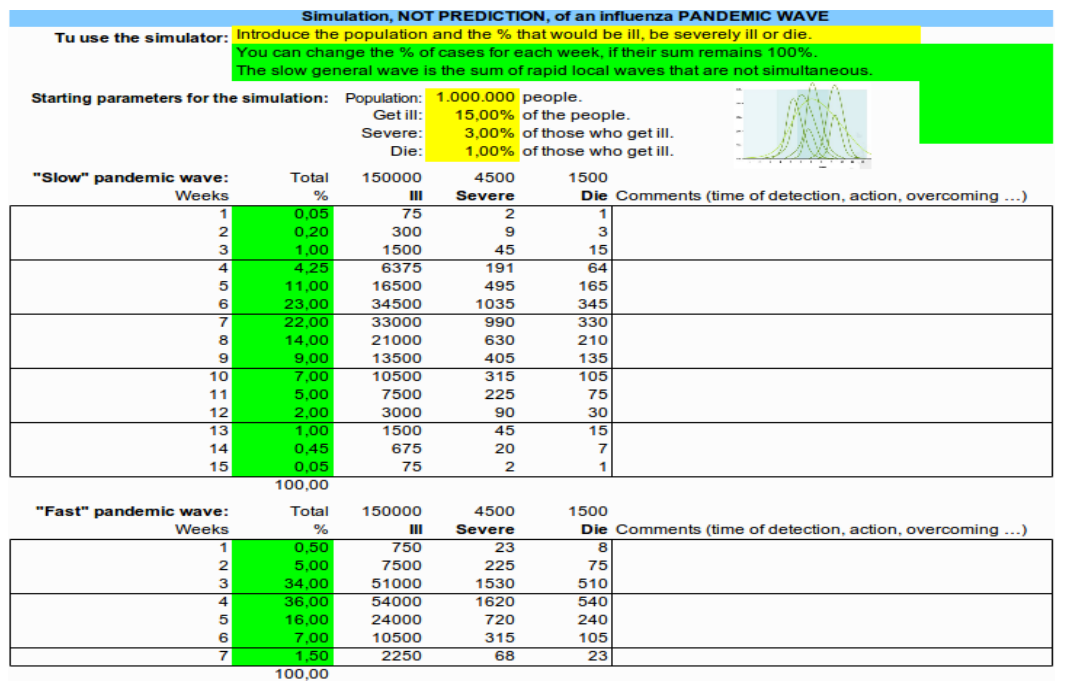
\includegraphics[width=15cm]{/figs/fig13.png}
\caption{Numerical simulation for a population of one million people, assuming that 15\% of the population will fall ill, that 3\% of those who do become sick will suffer severe illness, and that 1\% of the ill will die.}.
\end{figure}

\subsection{Templates}
Goal: An Integrated Needs Analysis Matrix (INAM) and the development of care plans.

Material: spreadsheet.

Contents:
\begin{itemize}
	\item Using SCIM-INAM.
	\item Health-care center template. In order to help each other in the process of planning and adaptation, centers may “anonymize” their plan documents even while they are in draft stage, deleting from copies data such as names and personal contact information, and share these drafts as they are developed, to be adapted as conditions require.
\end{itemize}

\subsection{Other causes of global systemic disruption}
Severe influenza pandemics are obviously not the only cause of global systemic disruption. Various entities pay attention to these risks\footnote{http://www.cabinetoffice.gov.uk/sites/default/files/resources/CO_NationalRiskRegister_2012_acc.pdf}, which can be classified according to their cause (biological, climatic and so on), scope (local, large, global), degree of complexity, duration and predictability. 

The analysis in this paper pertains to a severe pandemic: biological cause, global, complex, lasting from several months to more than a year, and unpredictable as to the time of onset, the specific nature of the virus, its effects and its evolution.

However, crises deriving from causes other than an influenza pandemic may also be addressed using some of the strategies mentioned in this document, with the exception of the sections devoted to prevention and treatment. Just by way of example:
\begin{itemize}
	\item If there is physical damage to the premises (earthquake or attack), SCIM's “workplace” section takes on an importance that is not necessarily great in a pandemic, however serious it may be.
	\item If the crisis is a climate one, we must pay attention to the effect of weather (SCIM's excessive heat or excessive cold) both on people (especially the most vulnerable) and on crops and animals, with consequent effects on food production.
\end{itemize}

\subsection{Macaronesian Islands}
This document has been produced to be useful for the islands of Macaronesia, which include the archipelagos of Azores, Canary Islands, Cape Verde, Madeira and the Savage Islands.

\begin{figure}[h]
\centering
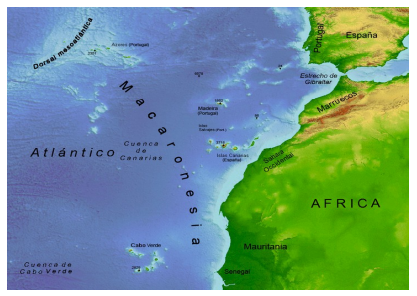
\includegraphics[width=10cm]{/figs/fig14.png}
\caption{Islands of Macaronesia. Source: Wikipedia}
\end{figure}

\begin{center}
\begin{tabular}{ | m{3cm} | m{3cm} | m{3cm} | m{3cm} | m{3cm} |}
 \hline
\textbf{Country} & \textbf{Archipelago} & \textbf{Inhabitants} & \textbf{If 30\% sick} & \textbf{If 1\% die}\\
 \hline
Spain & Canary Islands & 2,103,992 & 631,198 & 6,312 \\
 \hline
Cape Verde & Cape Verde & 499,796 & 149,939 & 1,499 \\
 \hline
Portugal & Madeira & 247,399 & 74,220 & 742 \\
 \hline
Portugal & Azores Islands & 245,374 & 73,612 & 736 \\
 \hline
 & & 3,096,561 & 928,968 & 9,290 \\
 \hline
\end{tabular}
\end{center}


\end{document}